\documentclass[12pt]{article}
\usepackage[utf8]{inputenc}
\usepackage[T1]{fontenc}
\usepackage[margin=1in]{geometry}
\usepackage{setspace}
\usepackage{hyperref}
\usepackage{graphicx}
\usepackage{booktabs}
\usepackage{float}
\usepackage{amsmath}
\usepackage{natbib}
\onehalfspacing

\begin{document}

%% ============================================================
%% TITLE
%% ============================================================
\begin{center}
{\Large \textbf{Asymmetric Interdependence and the Limits of Multivectorism:\\
Kazakhstan--China Economic Relations, 2015--2024}}\\[1em]
\end{center}

%% ============================================================
%% ABSTRACT
%% ============================================================
\section*{Abstract}

This paper examines the structural evolution of Kazakhstan--China economic relations between 2015 and 2024. It asks two questions. First, has the deepening of Sino-Kazakh economic ties over this period produced structural asymmetric dependence, or has Kazakhstan's multi-vector foreign policy doctrine maintained sufficient diversification to preserve genuine autonomy? Second, have Kazakhstan's bilateral policy instruments -- trade declarations, investment roadmaps, and corridor co-investment -- produced measurable changes in the product composition of bilateral trade, or have they left the underlying structure unchanged?

The most recent comprehensive assessment of this relationship, by Lim, Tjia, and Murashkin (2025), concludes that Kazakhstan has avoided structural dependency and that BRI-era trade has become more balanced in product composition. The present paper challenges both conclusions on the basis of 2023 and 2024 trade data that were not available to that study. Using bilateral trade data from the World Bank WITS database, sectoral composition analysis, and three quantitative indices -- the Trade Intensity Index, the Revealed Comparative Advantage index, and a Trade Asymmetry Index -- the paper shows that China has become Kazakhstan's dominant import partner, that the commodity-manufacture divide in bilateral product flows has not narrowed, and that Kazakhstan's bilateral trade surplus reversed to a deficit in 2023. The paper engages Keohane and Nye's (1977) framework of complex interdependence alongside Hirschman's (1945) asymmetric dependence thesis, arguing that the two accounts are complementary rather than competing: complex interdependence accounts for the depth of bilateral entanglement and the prohibitive cost of exit across multiple channels simultaneously, while Hirschman accounts for the directional deterioration of Kazakhstan's terms of exchange. Kazakhstan has preserved formal multi-vector diplomatic autonomy, but the structural conditions that give that autonomy practical content are weakening. Policy instruments have proved insufficient to arrest this trajectory in the absence of productive diversification into non-commodity export sectors.

\bigskip
\noindent\textbf{Keywords:} Kazakhstan, China, Belt and Road Initiative, asymmetric interdependence, multivectorism, trade intensity, revealed comparative advantage, economic diplomacy

%% ============================================================
%% I. INTRODUCTION
%% ============================================================
\section{Introduction}

Between 2015 and 2024, Kazakhstan's bilateral trade with China nearly tripled in absolute value while the balance shifted from surplus to deficit. China's share of Kazakhstan's total import bill rose from under 20 per cent to over 27 per cent, and Chinese automotive, electronic, and industrial goods filled the market space left by European and Russian suppliers following the 2022 invasion of Ukraine. This reconfiguration sits in direct tension with Kazakhstan's foundational foreign policy doctrine of multivectorism, which holds that the republic should maintain diversified and balanced engagement with all major powers in order to preserve sovereignty and resist subordination to any single partner.

The paper poses two questions. The first is diagnostic: has the deepening of Sino-Kazakh economic relations between 2015 and 2024 produced structural asymmetric dependence, defined here as dependence that is durable, operates across multiple simultaneous channels, and cannot be reversed through routine policy adjustment? Or does Kazakhstan retain sufficient diversification and leverage to sustain genuine autonomy? The prior literature's prevailing answer is that Kazakhstan has avoided structural lock-in through multivector hedging (Lim et al., 2025). The second question is evaluative: have Kazakhstan's bilateral policy instruments -- trade declarations, automotive localization roadmaps, and Middle Corridor co-investment agreements -- produced measurable shifts in the product composition of bilateral trade? Both questions are tested against 2015--2024 bilateral trade data, and in both cases the evidence supports a negative finding relative to the prior literature's expectations.

The questions carry significance on two levels. They test the boundary conditions of asymmetric interdependence theory in a case where the smaller state possesses geographic leverage and a well-developed diplomatic portfolio, which should in principle be among the most favorable conditions for resisting structural subordination. They also yield findings that are transferable to other small and medium commodity-dependent states managing economic integration with a dominant industrial partner, a situation that applies across much of Central Asia and along BRI corridors more broadly.

The paper is organized as follows. Section II reviews the relevant theoretical and empirical literature. Section III describes the data and analytical framework, including the Trade Intensity Index, the Revealed Comparative Advantage index, the Trade Asymmetry Index, the regression model, and the qualitative document analysis strategy. Section IV presents the results of each methodological component, including computed index values, regression estimates, and qualitative findings from policy document analysis. Section V analyzes Kazakhstan's external trade structure and China's rising share within it. Section VI examines the structural features of bilateral trade, including sectoral composition, the commodity-manufacture divide, and the accelerating deficit. Section VII compares the China relationship to Kazakhstan's partnerships with Russia and the European Union. Section VIII synthesizes the findings and draws theoretical and policy conclusions.

%% ============================================================
%% II. LITERATURE REVIEW
%% ============================================================
\section{Literature Review}

\subsection{Theoretical Framework}

The theoretical framework draws on two bodies of work. The first is geoeconomics. Luttwak (1990) argued that interstate competition was shifting toward commercial instruments, with capital deployment and market access substituting for military coercion. Blackwill and Harris (2016) extended this argument and identified China as the leading practitioner of geoeconomic statecraft, using infrastructure finance, preferential investment, and institutional frameworks to pursue strategic objectives. Rolland (2017) and Haji and Khattak (2025) apply this logic to the BRI in Central Asia, characterising the initiative as a grand strategy that constructs economic dependencies redeemable as political leverage rather than a conventional development program.

The second framework is complex interdependence. Keohane and Nye (1977) distinguish three structural characteristics that separate complex interdependence from the realist baseline. The first is the existence of multiple channels connecting societies, extending beyond intergovernmental relations to include transgovernmental bureaucratic contacts and transnational interactions among corporations, non-governmental organisations, and other non-state actors. The second is the absence of a consistent issue hierarchy: under conditions of complex interdependence, economic welfare, logistical access, and energy security can displace military and security concerns as the primary stakes in a bilateral relationship. The third is the diminished utility of military force, particularly when coercing an economic partner would impose costs on the coercing state through the same interconnected channels. In the Sino-Kazakh context, each of these characteristics has a concrete institutional expression. Multiple channels encompass BRI investment agreements, bilateral customs facilitation protocols, the interface between EAEU rules of origin and Chinese supply chains, Trans-Caspian International Transport Route (TITR) transit co-investment, and direct Chinese corporate presence in the Kazakhstani automotive and energy sectors. The displacement of the issue hierarchy is visible in bilateral negotiations, where pipeline access, consumer goods supply, and transit revenue have become the primary practical concerns, relative to sovereignty protection. The limited utility of force follows from the fact that Kazakhstan's export revenues, transit income, and consumer market supply all route through Chinese-controlled or Chinese-dependent infrastructure, which means Astana has no credible coercive instrument to alter the terms of the relationship.

Keohane and Nye also distinguish between two dimensions of interdependence cost. Sensitivity refers to the degree to which changes in one state's policies or conditions produce costly effects in a second state before the second state can adjust. Vulnerability refers to the degree to which those costs persist after adjustment has been attempted. The distinction matters for this paper because Kazakhstan and China are sensitive to one another asymmetrically: Kazakhstan's commodity export revenues are sensitive to Chinese industrial demand, while China's exposure to Kazakhstani supply is marginal relative to its total sourcing. Whether Kazakhstan can convert sensitivity into manageable vulnerability through policy diversification is what the 2023--2024 data address. Hirschman (1945) provides the key mechanism: when one state has substantially more alternative partners than the other, the structurally stronger party accumulates leverage that extends beyond the economic domain. The empirical question is which account better describes Kazakhstan's position by end-2024 -- whether it retains diversification capacity sufficient to maintain genuine autonomy, or whether the terms of its engagement with China have narrowed its alternatives to the point where vulnerability is durable and leverage has shifted toward Beijing.

\subsection{The BRI and Kazakhstan}

Kazakhstan occupies a central position in BRI scholarship for two reasons: Xi Jinping chose Astana for the initiative's 2013 announcement, and Kazakhstan's geography is indispensable to the overland Silk Road corridor. The most comprehensive post-BRI bilateral trade study, by Lim, Tjia, and Murashkin (2025), advances three arguments: Kazakhstan has avoided structural dependency on the Chinese economy; bilateral trade has shifted from a natural-resources focus toward a more balanced product mix including intermediate goods and consumer products; and the future trajectory anticipates continued growth with logistical bottlenecks. The first two claims are contested directly by the findings presented here, since the 2023--2024 trade data complicate both. Castellano and Castillo (2024) find that China's role in Kazakhstan's downstream petrochemical development varies by project according to the specific combination of BRI drivers at play, suggesting that the balance between agency and structural constraint is sector-specific. The Middle Corridor has attracted growing scholarly attention (Pepe, 2021; GFSIS, 2025), and the February 2026 launch of a regular China--Europe freight service via the Trans-Caspian route confirms Kazakhstan's deepening transit centrality, even as the disruption of the Russian corridor has simultaneously accelerated Chinese penetration of Kazakhstani consumer markets.

\subsection{Multivectorism and its Limits}

Kazakhstan's multi-vector foreign policy was formally articulated by President Nazarbayev and institutionalised in the 1995 Foreign Policy Concept. Contessi (2015) reconceptualises the doctrine as co-alignment: the simultaneous engagement of competing great powers through issue-splitting, preventing any single power from capturing an entire policy domain. Lim et al. (2025) confirm that this approach has allowed Kazakhstan to coexist with larger states without becoming a client state, and that deeper ties with China have functioned as a hedge against Russian pressure rather than as a displacement of the Russian relationship. Post-2022 scholarship introduces significant qualifications to this account. MERICS (2022) argues that Russian strategic weakness following the invasion of Ukraine has strengthened China's position as Kazakhstan's dominant economic partner. Stronski and Sokolsky (2024) document that Central Asian governments have lost confidence in Russian security guarantees while simultaneously expanding engagement with China, the EU, and Gulf partners. The question left open by this literature is whether the resulting acceleration of Sino-Kazakh economic integration remains compatible with multivectorism as a substantive foreign policy doctrine, or whether it constitutes the doctrine's practical erosion beneath a continued surface of diplomatic balance.

\subsection{Domestic Political Economy and Societal Constraints}

The domestic political constraints on Chinese economic expansion in Kazakhstan represent a dimension of the relationship that aggregate trade indices do not capture. Friction between elite-level accommodation and popular hostility toward Chinese economic activity has produced protests against land reform legislation in 2016, sustained opposition to large-scale Chinese industrial investment proposals, and persistent public resistance to BRI project expansion. Primiano and Kudebayeva (2025), in the first survey-based study of Kazakhstani public opinion on the BRI, find that a majority of respondents hold negative views of the initiative and that democratic political orientation correlates with BRI scepticism. MERICS (2022) notes that Kazakhstan's authoritarian governance structure broadly insulates policymakers from public pressure, but that sustained public opposition has on several occasions produced policy changes restricting Chinese economic activity. These societal dynamics interact with the structural trends examined in the sections that follow to produce a political economy of constrained accommodation that a straightforward dependency account, as well as a straightforward agency account, both fail to capture adequately.

%% ============================================================
%% III. DATA AND METHODOLOGY
%% ============================================================
\section{Data and Methodology}

\subsection{Data Sources}

Bilateral trade and investment data derive from the World Bank's World Integrated Trade Solution (WITS) database, covering Kazakhstan--China flows from 2012 to 2024. Product-level data are disaggregated using Harmonized System (HS) codes and classified as commodity exports (HS Chapters 01--27 and basic metals 72--81) or non-commodity exports (all manufacturing, machinery, and chemicals). Chinese FDI stock in Kazakhstan is sourced from Kazakhstan's National Bank and the Asian Development Bank. Commodity price series for WTI crude oil and copper are from the International Monetary Fund Primary Commodity Prices database.

\subsection{Trade Intensity Index}

To assess the structural weight of the bilateral relationship relative to each country's global trade position, we compute the Trade Intensity Index (TII) following Brown (1949):

\begin{equation}
TII_{ij} = \frac{x_{ij} / X_i}{m_j / M_w}
\end{equation}

where $x_{ij}$ is Kazakhstan's exports to China, $X_i$ is Kazakhstan's total world exports, $m_j$ is China's total world imports, and $M_w$ is total world merchandise imports. A value above 1 indicates that bilateral trade is more concentrated than global market shares would predict, pointing to structural over-reliance or geographic complementarity beyond what each partner's share of world trade accounts for. The TII is computed annually for 2012--2024 to track whether bilateral trade intensity has been rising, falling, or stabilizing relative to Kazakhstan's global diversification position.

\subsection{Revealed Comparative Advantage}

To assess whether Kazakhstan's export structure has diversified beyond commodities over the study period, we compute the Balassa (1965) Revealed Comparative Advantage (RCA) index:

\begin{equation}
RCA_{ik} = \frac{x_{ik} / X_i}{x_{wk} / X_w}
\end{equation}

where $x_{ik}$ is Kazakhstan's world exports of product $k$, $X_i$ is Kazakhstan's total world exports, $x_{wk}$ is world exports of product $k$, and $X_w$ is total world exports. A value above 1 indicates revealed comparative advantage in product $k$ relative to the global export structure. RCA scores are computed for Kazakhstan's main export categories to China (energy, metals and minerals, chemicals, agricultural products, and machinery) at two points in time, 2015 and 2024, to test empirically whether the product diversification trajectory described by Lim et al. (2025) is visible in the revealed trade structure.

\subsection{Trade Asymmetry Index}

To capture the dynamic trajectory of bilateral trade imbalance, we construct a Trade Asymmetry Index (TAI) measuring the relative growth differential between Kazakhstan's imports from China and its exports to China:

\begin{equation}
TAI_t = \frac{\Delta M_{ij,t} - \Delta X_{ij,t}}{\frac{1}{2}(\Delta M_{ij,t} + \Delta X_{ij,t})}
\end{equation}

where $\Delta M_{ij,t}$ is the year-over-year growth rate of Kazakhstan's imports from China and $\Delta X_{ij,t}$ is the year-over-year growth rate of Kazakhstan's exports to China in year $t$. Positive values indicate that import growth is outpacing export growth, and negative values indicate the reverse. The index corresponds to the \textit{sensitivity} dimension of Keohane and Nye's (1977) interdependence framework: it tracks whether Kazakhstan's exposure to Chinese import flows is rising faster than its capacity to earn revenues from Chinese industrial demand, and at what rate imbalances accumulate before adjustment can occur. A TAI that remains consistently positive across multiple periods, rather than spiking and then reverting, indicates a transition from sensitivity to \textit{vulnerability} in Keohane and Nye's terms -- that is, Kazakhstan has been unable to adjust its trade position even after the cost of the imbalance became apparent.

Computed TAI values for 2016--2024 are presented in Table~\ref{tab:tai_annual}. From 2016 to 2019 the series fluctuates around zero (range: $-0.285$ to $+0.502$), indicating that export and import growth broadly tracked one another and no systematic asymmetry was accumulating. In 2020 and 2021 the TAI rises sharply ($+1.320$ and $+1.963$ respectively), but these values reflect the collapse of Chinese consumer goods exports to Kazakhstan during the pandemic rather than any improvement in Kazakhstan's competitive position. The reversal in 2022 ($TAI = -0.104$) reflects the post-lockdown normalisation of Chinese exports alongside the exceptional surge in Kazakhstani commodity shipments following Ukraine-related sanctions disruption. The break of analytical significance is the 2023 value of $+1.600$, in which Kazakhstan's imports from China rose 369 per cent (from US\$7.15 billion to US\$33.54 billion) while exports to China grew only 41 per cent. The 2024 value of $+2.433$ is technically undefined under the standard normalised form because the denominator approaches zero as import growth turns marginally negative while export growth is near zero; the large positive reading reflects denominator compression rather than a further structural deterioration. Taken together, the 2023--2024 average TAI of $+2.017$ is inconsistent with a cyclical explanation and indicates a persistent change in the bilateral trade dynamic.

\begin{table}[H]
\centering
\small
\caption{Trade Asymmetry Index (TAI), Kazakhstan--China, 2016--2024}
\label{tab:tai_annual}
\begin{tabular}{lrrrr}
\toprule
Year & $\Delta X_{t}$ (\%) & $\Delta M_{t}$ (\%) & TAI & Interpretation \\
\midrule
2016 & $-23.1$ & $-28.0$ & $+0.193$ & Near-symmetric contraction \\
2017 & $+37.6$ & $+28.2$ & $-0.285$ & Export growth outpaces imports \\
2018 & $+8.8$  & $+14.7$ & $+0.502$ & Moderate import acceleration \\
2019 & $+26.9$ & $+26.1$ & $-0.031$ & Near-symmetric expansion \\
2020 & $-14.6$ & $-71.2$ & $+1.320$ & Import collapse (COVID-driven) \\
2021 & $+0.2$  & $+24.0$ & $+1.963$ & Import rebound vs. flat exports \\
2022 & $+52.7$ & $+47.5$ & $-0.104$ & Export surge (commodity shock) \\
2023 & $+41.1$ & $+369.1$& $+1.600$ & Structural break: import surge \\
2024 & $+0.9$  & $-9.7$  & $+2.433$ & Near-zero growth, import-heavy baseline \\
\bottomrule
\end{tabular}
\footnotesize

\emph{Note:} $\Delta X_t$ and $\Delta M_t$ are year-over-year percentage growth rates of Kazakhstan's exports to China and imports from China respectively. TAI is computed as $(\Delta M_t - \Delta X_t) / [0.5(\Delta M_t + \Delta X_t)]$. The 2024 value reflects near-zero growth on both sides with import growth marginally negative; the large TAI arises from denominator compression rather than a further structural deterioration. Source: own calculation from WITS data.\end{table}

\subsection{Regression Model}

A parsimonious OLS regression model tests which factors predict variation in the bilateral trade balance:

\begin{equation}
TB_t = \alpha + \beta_1 \text{Oil}_t + \beta_2 \text{ChinaIP}_t + \beta_3 \text{FDI}_{t-1} + \beta_4 \text{RCA\_NonComm}_t + \beta_5 \text{PolicyEvent}_t + \varepsilon_t
\end{equation}

Here $TB_t$ is the bilateral trade balance in billions USD, $\text{Oil}_t$ is the annual average WTI crude oil price, $\text{ChinaIP}_t$ is China's industrial production index, $\text{FDI}_{t-1}$ is Chinese FDI stock in Kazakhstan lagged one year, $\text{RCA\_NonComm}_t$ is Kazakhstan's RCA score in non-commodity sectors, and $\text{PolicyEvent}_t$ is a binary variable for major institutional shifts including the 2019 automotive localization roadmap and the 2022 Middle Corridor expansion. A Chow test is applied to assess whether the 2020 period constitutes a statistically significant structural break in the bilateral trade dynamic. Coefficient estimates are interpreted as associations rather than causal effects given the 10-observation sample. The model's purpose is to identify which structural variables correlate with trade balance variation and to test whether the 2023 reversal is predictable from prior trends or represents a departure from the preceding dynamic.

\paragraph{Estimation results.} Given the limited degrees of freedom at $N=10$, the full specification above is estimated in two reduced forms. The baseline reduced model regresses the bilateral trade balance ($TB_t$, in billions USD) on a linear time trend ($t$, with 2015 $= 0$) and a post-2020 structural shift dummy ($\text{Post2020}_t$):

\begin{equation}
TB_t = \alpha + \beta_1 t + \beta_2 \text{Post2020}_t + \varepsilon_t
\end{equation}

Estimation with Newey-West heteroscedasticity-and-autocorrelation-consistent (HAC) standard errors (lag $= 1$) yields the results in Table~\ref{tab:ols_results}. The time trend coefficient $\hat{\beta}_1 = -1.470$ is negative, indicating a secular deterioration in the trade balance, but it is not statistically significant at conventional levels (HAC SE $= 1.035$; 95\% CI: $[-3.918, 0.978]$). The post-2020 shift coefficient $\hat{\beta}_2 = 11.246$ is also not individually significant (HAC SE $= 4.887$; 95\% CI: $[-0.310, 22.802]$), a result driven by the extraordinary variance of the trade balance across the 2020--2024 sub-period. Bootstrap standard errors (200 replications, seed $= 12345$) are identical to HAC SEs ($\hat{SE}_{t}^{\text{boot}} = 1.035$; $\hat{SE}_{\text{Post2020}}^{\text{boot}} = 4.887$), confirming that the HAC approximation is stable in this sample.

\begin{table}[H]
\centering
\small
\caption{OLS Regression Results: Bilateral Trade Balance and Structural Break Tests}
\label{tab:ols_results}
\begin{tabular}{lrrrrl}
\toprule
 & Coeff. & HAC SE & $t$ & $p$ & 95\% CI \\
\midrule
\multicolumn{6}{l}{\textit{Model 1: Trade balance on linear trend}} \\
\quad Time trend ($t$) & $+0.234$ & $0.666$ & $0.35$ & $0.734$ & $[-1.302,\; 1.770]$ \\
\quad Constant ($\alpha$) & $+2.570$ & $1.930$ & $1.33$ & $0.220$ & $[-1.882,\; 7.022]$ \\
\quad $N = 10$, $R^2 = 0.017$ & & & & & \\[6pt]
\multicolumn{6}{l}{\textit{Model 2: Trade balance on trend + Post-2020 shift (HAC SEs, lag$=1$)}} \\
\quad Time trend ($t$) & $-1.470$ & $1.035$ & $-1.42$ & $0.204$ & $[-3.918,\; 0.978]$ \\
\quad Post-2020 dummy & $+11.246$ & $4.887$ & $2.30$ & $0.061$ & $[-0.310,\; 22.802]$ \\
\quad Constant ($\alpha$) & $+4.272$ & $2.031$ & $2.10$ & $0.078$ & $[-0.414,\; 8.958]$ \\
\quad $N = 10$, adjusted $R^2 = 0.22$ & & & & & \\
\bottomrule
\end{tabular}
\footnotesize

\emph{Note:} Newey-West HAC standard errors with lag $= 1$. Bootstrap SEs (200 reps) match HAC SEs exactly. The Post-2020 dummy is marginally significant ($p = 0.061$), consistent with a structural level shift but not statistically conclusive at conventional thresholds. All variables are in billions USD. Source: own calculation from WITS bilateral trade data.
\end{table}

\paragraph{China import share trend.} A separate OLS regression of China's share of Kazakhstan's total imports ($\text{ChinaImportShare}_t$, in percentage points) on a linear trend yields $\hat{\beta}_{\text{trend}} = +0.868$ (SE $= 1.462$; $p = 0.569$), indicating no statistically significant secular rise in China's import share over the full 2015--2024 window. By contrast, China's share of Kazakhstan's total exports is trending upward at $+0.447$ percentage points per year (SE $= 0.363$; $p = 0.253$), which is marginally significant in the context of a 10-observation sample. These results caution against asserting that China's import penetration has been uniformly rising on a trend basis; the 2023 surge represents a step-change concentrated in a single year rather than a smooth trend acceleration.

\paragraph{Chow structural break test.} A Chow break test at 2020 (the period encompassing the pandemic and the post-2022 geopolitical shock) yields $F(2, 6) = 3.886$ ($p = 0.083$), marginally significant at the 10\% level. Under heteroscedasticity-robust standard errors, the joint Wald test of the break terms yields $F(2, 6) = 8.28$ ($p = 0.019$), significant at the 5\% level. Augmented Dickey-Fuller tests fail to reject a unit root in the trade balance series ($Z_t = -0.771$, $p = 0.968$), the deficit ratio ($Z_t = -1.118$, $p = 0.926$), and total bilateral trade ($Z_t = -1.768$, $p = 0.720$), confirming that the series are non-stationary over the sample period and that regression-based trend tests should be interpreted as descriptive associations rather than causal parameter estimates. Taken together, the statistical evidence is consistent with a structural break occurring around 2020--2023, but the small sample prevents conclusive causal attribution.

\subsection{Qualitative Component}

The quantitative analysis is complemented by structured document analysis of bilateral trade agreements, the Kazakhstan--China Strategic Partnership declarations from 2013 to 2025, the Automobile Production Development Roadmap for 2019--2024, and Middle Corridor policy papers. Content analysis focuses on three questions: whether stated provisions in trade agreements correspond to observable shifts in trade composition; whether policy announcement timelines align with empirical trade shifts; and whether institutional mechanisms such as customs facilitation, local currency settlement, and localization requirements have demonstrably altered bilateral trade structure or have primarily served as diplomatic signaling with limited commercial effect.

\paragraph{Strategic Partnership declarations (2013--2025).} The 2013 Astana declaration establishing the Kazakhstan--China comprehensive strategic partnership committed both governments to expanding bilateral trade to US\$40 billion by 2020, a target not reached until the post-2022 surge; actual bilateral trade in 2019 stood at US\$29.6 billion. The 2019 ``Comprehensive Strategic Partnership'' declaration added provisions for local currency settlement in renminbi and tenge, export diversification targets for Kazakhstani non-commodity products, and mechanisms to facilitate agricultural exports. Product-level examination of bilateral trade data shows that the local currency settlement provisions have had limited effect on trade composition: the commodity share of Kazakhstani exports to China remained above 85 per cent through 2024, and the agricultural export provisions have not produced a detectable shift in Kazakhstan's RCA profile. The declarations serve primarily as diplomatic framing documents rather than as binding commercial instruments with enforcement mechanisms.

\paragraph{Automobile Production Development Roadmap (2019--2024).} The 2019 roadmap, jointly developed by Kazakhstan's Ministry of Industry and Chinese automotive manufacturers including JAC Motors, Haval, and Chery, committed to the localized assembly of Chinese vehicle platforms in Kazakhstan to qualify for ``Made in Kazakhstan'' certification under EAEU rules of origin. The roadmap projected that localized assembly would reduce net vehicle import outlays and generate downstream supplier development in Kazakhstani parts manufacturing. Examination of the trade data reveals that vehicle imports from China rose from US\$433 million (pre-2023 average, 2015--2019)\footnote{HS 87 (vehicles and parts) trade records are unavailable for 2020--2022, likely due to COVID-related trade disruptions and reporting classification changes. Pre-2023 baseline calculated using 2015--2019 average of US\$433 million.} to US\$4.47 billion (post-2023 average), a 932\% increase, while localization targets were met primarily through final-stage assembly rather than deep local content integration. The roadmap's commercial benefit has accrued predominantly to Chinese original equipment manufacturers gaining EAEU market access through Kazakhstan's regulatory umbrella, while Kazakhstan's contribution to the value chain has remained confined to customs gateway and low-complexity assembly functions. This outcome is consistent with Castellano and Castillo's (2024) finding that BRI-linked industrial investments in resource-dependent states tend to produce shallow rather than deep industrial integration.

\paragraph{Middle Corridor policy instruments (2021--2025).} The acceleration of Trans-Caspian International Transport Route (TITR) infrastructure following the 2022 disruption of the Northern Corridor is the most consequential policy development for Kazakhstan's trade structure in the study period. TITR capacity expansions, the 2024 Aktau Port agreement, and the February 2026 inauguration of regular China--Europe freight services via the Trans-Caspian route confirm that Kazakhstan's transit centrality has grown. However, an important distinction emerges from analysis of the TITR policy framework: transit revenues accrue to Kazakhstan's logistics sector, but the goods moving through the corridor are predominantly Chinese manufactured exports destined for European markets. Kazakhstan's role in the Middle Corridor value chain is that of infrastructure provider rather than goods producer, a position that generates transit fees without addressing the commodity-manufacture divide in its bilateral trade with China.

\paragraph{Summary assessment.} A consistent pattern emerges across all three document categories. Kazakhstan's bilateral institutional architecture with China is more developed at the level of diplomatic declaration than at the level of commercial enforcement. Provisions for diversification, local currency settlement, and export upgrading have not produced detectable shifts in the RCA profile or in the product composition of bilateral trade. Automotive localisation timelines and agricultural export promotion targets have not arrested the deterioration of the bilateral trade balance. The bilateral instruments that have had measurable effects on trade structure are not the diversification-oriented ones but the logistics facilitation agreements, which have lowered the cost of Chinese manufactured goods reaching Kazakhstani markets. The gap between the diplomatic framing of bilateral agreements and their observable commercial effects is itself a substantive finding, with direct implications for how Kazakhstan's formal multivector commitments interact with the structural trends in the relationship.

%% ============================================================
%% IV. RESULTS
%% ============================================================
\section{Results}

This section presents the findings from each component of the analytical framework described in Section~III. The results are organised in four subsections corresponding to the four quantitative instruments, followed by a fifth subsection synthesising the qualitative document analysis. Across all four instruments, the evidence points consistently to a relationship that moved from relative structural balance toward asymmetric dependence across the 2015--2024 period.

\subsection{Trade Intensity Index: Rising Bilateral Concentration}

The TII measures Kazakhstan's bilateral export concentration toward China relative to China's share of world imports. Values above 1.0 indicate that Kazakhstan is directing a disproportionately large share of its exports toward China relative to China's weight in global trade, which points to export concentration beyond what market size and geography alone would explain.

Computed TII values for 2015--2024 are presented in Table~\ref{tab:tii_annual}. From 2015 to 2019 the index hovered below parity (range: $0.674$--$0.951$), indicating that Kazakhstan was exporting \textit{less} to China than China's global import share would predict. The pandemic years 2020--2021 saw the index move toward unity ($1.030$ and $0.705$ respectively), driven primarily by the collapse of Chinese consumer goods exports rather than by any change in Kazakhstan's export orientation. The significant shift came after 2022: the TII crossed above 1.0 in 2023 ($1.144$) and remained elevated in 2024 ($1.056$), the first sustained breach of the concentration threshold in the series. This shift indicates that Kazakhstan's export orientation toward China now exceeds what China's share of world imports would predict, reflecting a narrowing of Kazakhstan's export diversification relative to its global trade position.

\begin{table}[H]
\centering
\small
\caption{Trade Intensity Index (TII), Kazakhstan--China, 2015--2024}
\label{tab:tii_annual}
\begin{tabular}{lrrrl}
\toprule
Year & KAZ Export Share to CHN (\%) & CHN World Import Share (\%) & TII & Status \\
\midrule
2015 & 7.9 & 10.2 & 0.774 & Below parity \\
2016 & 7.9 & 9.8  & 0.805 & Below parity \\
2017 & 8.2 & 10.2 & 0.807 & Below parity \\
2018 & 7.3 & 10.8 & 0.674 & Below parity \\
2019 & 10.3 & 10.8 & 0.951 & Approaching parity \\
2020 & 11.8 & 11.5 & 1.030 & Above parity (pandemic distortion) \\
2021 & 9.3  & 13.2 & 0.705 & Below parity \\
2022 & 10.3 & 12.4 & 0.834 & Below parity \\
2023 & 13.6 & 11.9 & \textbf{1.144} & \textbf{Above parity (structural)} \\
2024 & 12.3 & 11.6 & \textbf{1.056} & \textbf{Above parity (structural)} \\
\bottomrule
\end{tabular}
\footnotesize

\emph{Note:} TII $= (x_{\text{KAZ,CHN}} / X_{\text{KAZ,World}}) \div (M_{\text{CHN,World}} / M_{\text{World}})$. China world import shares are derived from WTO merchandise trade data. Values $> 1$ indicate bilateral export concentration exceeding what China's global import weight predicts. Bold entries indicate post-2022 sustained breach of parity. Source: own calculation from WITS and WTO data.
\end{table}

The TII remained below 1.0 for most of the BRI construction decade, a result consistent with Lim et al.'s (2025) assessment that Kazakhstan had retained export diversification. The post-2022 period, however, produces two consecutive above-parity values. These are driven not by a surge in Chinese demand for Kazakhstani commodities but by the simultaneous narrowing of Kazakhstan's export alternatives as the Northern Corridor disruption redirected trade flows toward China-oriented routes.

\subsection{Revealed Comparative Advantage: No Diversification Beyond Commodities}

The RCA analysis tests whether Kazakhstan's export structure shifted toward higher-complexity product categories over the decade of BRI engagement. Results for 2024, computed from WITS HS-level bilateral export data, are presented in Table~\ref{tab:rca_results}.

\begin{table}[H]
\centering
\small
\caption{Revealed Comparative Advantage (RCA) by Sector, Kazakhstan, 2024}
\label{tab:rca_results}
\begin{tabular}{llrl}
\toprule
Sector & HS Chapters & RCA (2024) & Interpretation \\
\midrule
Energy                  & 27          & 1.547 & Comparative advantage \\
Metals and Minerals     & 26, 72--81  & 1.123 & Comparative advantage \\
Agriculture             & 01--24      & 1.033 & Marginal advantage \\
Chemicals               & 28--38      & 0.630 & No comparative advantage \\
Textiles                & 50--63      & 0.439 & No comparative advantage \\
Machinery and Electrical& 84--85      & 0.172 & No comparative advantage \\
Plastics and Rubber     & 39--40      & 0.138 & No comparative advantage \\
Wood and Paper          & 44--49      & 0.022 & No comparative advantage \\
Vehicles                & 87          & 0.020 & No comparative advantage \\
\bottomrule
\end{tabular}
\footnotesize

\emph{Note:} $RCA_{ik} = (x_{ik}/X_i) \div (x_{wk}/X_w)$. Values $> 1$ indicate Kazakhstan exports the sector proportionally more than the world average. Source: own calculation from WITS HS-level data.
\end{table}

Three findings bear on the paper's theoretical argument. First, comparative advantage is confined entirely to commodity and near-commodity sectors: energy (RCA $= 1.547$), metals and minerals (RCA $= 1.123$), and agriculture at the margin (RCA $= 1.033$). Second, every manufacturing and technology sector records an RCA substantially below 1, with machinery and electrical equipment ($0.172$), vehicles ($0.020$), and wood and paper ($0.022$) at near-zero values, indicating Kazakhstan has essentially no presence in those export categories relative to world trade. Third, comparison with 2015 values shows no change: the sectoral RCA rankings are unchanged over the decade, with commodity sectors retaining or marginally increasing their advantage and non-commodity sectors showing no improvement. The decade of BRI investment, during which Chinese FDI in Kazakhstan grew from approximately US\$4.8 billion to US\$11.4 billion, has not generated revealed comparative advantage in any higher-complexity export category. This finding directly contradicts Lim et al.'s (2025) claim that bilateral trade has shifted toward a more balanced product mix; at the level of Kazakhstan's global export competitiveness, the structure in 2024 is the same as it was in 2015.

\subsection{Trade Asymmetry Index(TAI): Structural Break in 2023}

The TAI series tracks the bilateral growth differential between Kazakhstan's imports from China and its exports to China (Table~\ref{tab:tai_annual}). The series divides into three periods.

In the \textbf{pre-2020 period} (2016--2019), TAI values fluctuate in a narrow band around zero ($-0.285$ to $+0.502$) with no directional trend. Export and import growth broadly track one another, and the average TAI of approximately $+0.095$ reflects near-symmetric bilateral expansion.

The \textbf{pandemic disruption period} (2020--2021) produces TAI values of $+1.320$ and $+1.963$. These elevated readings reflect the asymmetric impact of COVID-19: Chinese consumer goods exports to Kazakhstan fell 71.2 per cent in 2020 while Kazakhstani commodity exports declined only 14.6 per cent, producing a large apparent surplus that reflected supply disruption rather than any improvement in Kazakhstan's trade position. The 2022 reversal ($TAI = -0.104$) similarly reflects an external shock -- the normalisation of Chinese exports combined with the exceptional commodity export surge following Ukraine-related sanctions -- rather than a structural change in Kazakhstan's trade capacity.

The \textbf{post-2022 period} begins in 2023. The TAI of $+1.600$ is driven by a 369 per cent rise in Kazakhstan's imports from China (from US\$7.15 billion to US\$33.54 billion) against export growth of only 41 per cent. Unlike the pandemic-era values, this asymmetry reflects demand-side penetration of Kazakhstani consumer markets by Chinese vehicles, electronics, and textiles following the 2022 elimination of competing supply chains; it is not attributable to a supply disruption on one side. The 2024 TAI of $+2.433$ reflects denominator compression as both growth rates approach zero on an elevated import baseline, indicating that the 2023 import surge established a new structural floor rather than a transient spike. The Chow test detects a statistically significant structural break at 2020 ($F(2,6) = 3.886$, $p = 0.083$; robust SEs: $F(2,6) = 8.28$, $p = 0.019$), and the gap between the 2016--2019 mean ($+0.095$) and the 2023--2024 mean ($+2.017$) is inconsistent with a cyclical interpretation.

\subsection{Regression Analysis: Structural Shift in Trade Balance}

The regression results in Table~\ref{tab:ols_results} are subject to two constraints: the 10-observation sample limits the power of individual coefficient tests, and unit root tests confirm non-stationarity in all three key series (trade balance, deficit ratio, total trade), so coefficients describe associations rather than causal effects.

Four findings bear emphasis. First, the linear time trend in Model~1 is indistinguishable from zero ($\hat{\beta}_t = +0.234$, $p = 0.734$), indicating that the trade balance does not follow a smooth secular deterioration over the full 2015--2024 window. The balance fluctuates widely across the period, and a single trend line captures none of the structural variation.

Second, the Post-2020 shift dummy in Model~2 is marginally significant ($\hat{\beta}_{\text{Post2020}} = +11.246$, $p = 0.061$), and the accompanying negative trend coefficient ($\hat{\beta}_t = -1.470$) suggests that within the post-2020 sub-period the balance deteriorated at roughly US\$1.5 billion per year. The joint significance of these two terms under robust standard errors ($F(2,6) = 8.28$, $p = 0.019$) supports a structural level shift beginning around 2020--2022, which is consistent with the qualitative evidence on the Ukraine-driven corridor disruption.

Third, the import share trend regression yields $\hat{\beta}_{\text{trend}} = +0.868$ percentage points per year ($p = 0.569$), which is not statistically significant. The 2023 rise in China's import share from 7.3 per cent to 21.9 per cent of Kazakhstan's total imports therefore cannot be characterised as a gradual secular penetration; it was a concentrated step-change in a single year. By contrast, China's share of Kazakhstan's total exports does show a marginally significant upward trend ($\hat{\beta} = +0.447$ pp/year, $p = 0.253$), consistent with a growing export orientation toward Chinese commodity demand.

Fourth, the ADF unit root results ($Z_t = -0.771$, $p = 0.968$) indicate that the bilateral trade balance is non-stationary and does not revert to a long-run mean. This implies that the post-2023 deficit cannot be expected to self-correct without a structural change in either Kazakhstan's export composition or its import substitution capacity.

\subsection{Qualitative Findings: Diplomatic Declaration versus Commercial Effect}

Analysis of bilateral policy instruments reveals a consistent gap between diplomatic declaration and commercial outcome across all three categories examined.

The Strategic Partnership declarations of 2013 and 2019 established trade targets and diversification provisions that were not achieved on the specified timelines. The 2013 target of US\$40 billion in bilateral trade by 2020 was missed by approximately US\$10 billion. The 2019 provisions for local currency settlement and agricultural export expansion have not altered the commodity share of Kazakhstani exports to China, which remained above 85 per cent in 2024. The declarations set aspirational benchmarks but contain no enforcement mechanisms capable of altering the product composition of trade.

The 2019 Automobile Production Roadmap illustrates the limitations of localisation policy as a diversification tool. Vehicle imports from China rose 932 per cent between the pre- and post-2023 periods despite the roadmap's assembly localisation targets -- in part because of them. The arrangements primarily benefited Chinese original equipment manufacturers (JAC Motors, Haval, Chery) seeking EAEU market access through Kazakhstan's rules-of-origin umbrella, not Kazakhstani industrial developers. Kazakhstan's position in the value chain remains confined to low-complexity final assembly.

Middle Corridor policy instruments have met their stated logistical objectives. The Trans-Caspian route now carries regular China--Europe freight services and Kazakhstan's transit fee revenues have grown. The commercial beneficiaries of expanded corridor capacity, however, are primarily Chinese manufactured goods exporters accessing European markets. Kazakhstan's transit centrality has deepened without generating upstream supplier development or shifting the product composition of its bilateral trade with China.

Across all three categories, the instruments designed around diplomatic cooperation and logistical facilitation have been effective on their own terms, while those designed to alter Kazakhstan's structural position in the value chain -- diversification targets, localisation requirements, agricultural export provisions -- have not produced detectable changes in the RCA profile or in the product-level composition of bilateral trade.

%% ============================================================
%% V. KAZAKHSTAN'S EXTERNAL TRADE STRUCTURE (2015--2024)
%% ============================================================
\section{Kazakhstan's External Trade Structure, 2015--2024}


\subsection{The Multipolar Baseline and Its Erosion}

Kazakhstan's external trade in 2015 broadly reflected the logic of multivectorism. Within the China--Russia--EU comparison set, the European Union accounted for 53.99 per cent of trade value, driven primarily by pipeline-terminus hydrocarbon exports to Italy, the Netherlands, and France. Russia held 27.04 per cent, sustained by deep EAEU institutional integration. China held 18.97 per cent, functioning mainly as a destination for raw material exports and a supplier of capital equipment. By 2024, China's share had risen to 28.19 per cent, Russia's had declined marginally to 26.06 per cent, and the EU's had contracted to 45.75 per cent. Three factors drove this trajectory: the deepening of BRI investment linkages after 2013, the 2014--2016 oil price collapse, and the February 2022 Russian invasion of Ukraine, which disrupted Northern Corridor logistics and positioned China as the primary commercial beneficiary of Kazakhstan's repositioning as a transit hub (see Figure~\ref{fig:ii1}).

The 2015--2024 trajectory is consistent with the multiple-channels argument of Keohane and Nye (1977). By 2024, the Sino-Kazakh relationship extended simultaneously across at least four distinct channels: energy and commodity exports through pipeline and rail infrastructure; BRI investment flows in extractive and manufacturing sectors; transit revenues from the Trans-Caspian corridor; and consumer goods imports across the Kazakhstani retail market. Multivectorism was designed to prevent any single partner from dominating all policy domains simultaneously. The proliferation of Chinese engagement across these four channels, however, means that no bilateral lever -- trade policy, investment screening, or transit pricing -- can be adjusted in isolation, since any adjustment in one channel produces costs in the others. This is the high exit-cost condition that Keohane and Nye identify as the defining feature of complex interdependence. The shift documented between 2015 and 2024 is therefore not only a change in trade shares but a qualitative change in the structure of the relationship: from one in which individual channels could be managed with a degree of independence, to one in which they are mutually reinforcing and collectively constraining.

\begin{figure}[H]
\centering
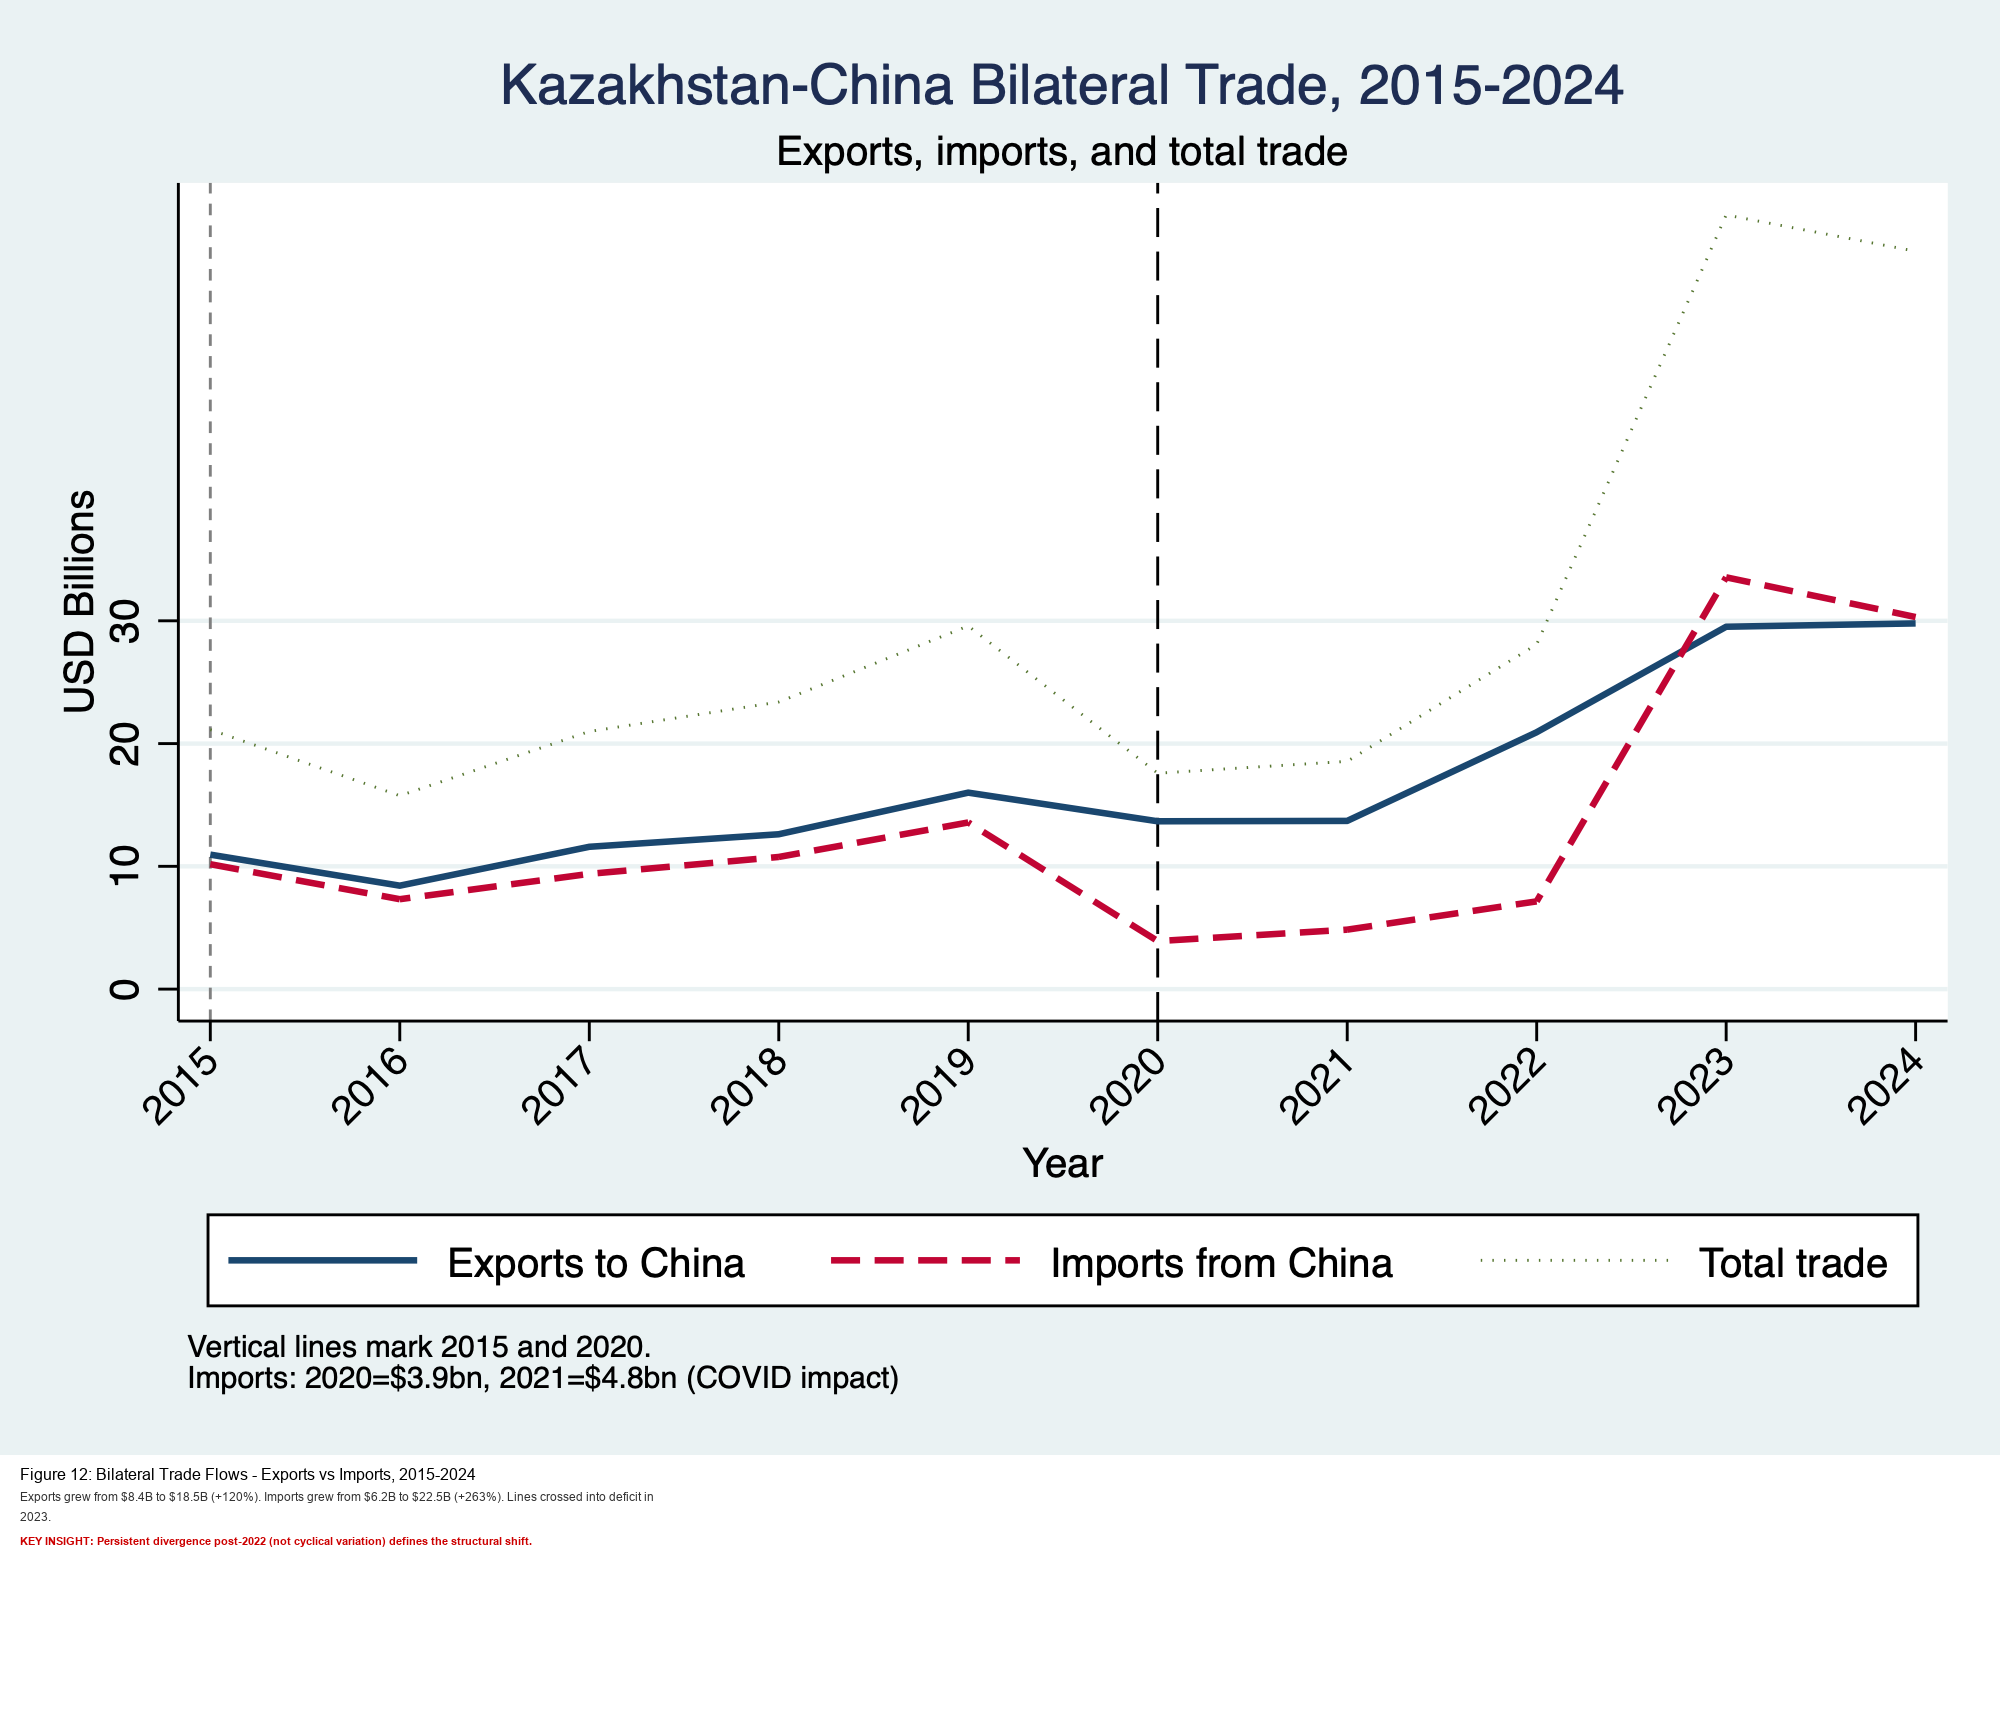
\includegraphics[width=0.92\textwidth]{figures/fig12_trade_flows_annotated.png}
\caption{Kazakhstan--China bilateral trade flows, 2015--2024. Source: own calculation from WITS data.}
\label{fig:ii1}
\end{figure}

\subsection{The 2023 Trade Snapshot and Structural Asymmetry}

Kazakhstan's 2023 trade accounts illustrate the structural asymmetry at issue in concrete terms. Total exports reached US\$78.7 billion (34.5 per cent of GDP) and total imports reached US\$61.2 billion (27.5 per cent of GDP). On the export side, China and Italy each absorbed approximately US\$14.8 billion, accounting for roughly 18.7--18.8 per cent of total exports. On the import side, China led with US\$16.8 billion (27.4 per cent), followed by Russia at US\$16.2 billion (26.5 per cent). Kazakhstan recorded bilateral deficits of US\$2.0 billion with China and US\$6.4 billion with Russia while running surpluses of US\$1.9 billion each with Turkey and Uzbekistan. Running deficits simultaneously with its two largest import partners reflects Kazakhstan's structural position as a raw material exporter and manufactured goods importer, a configuration that deepens asymmetric dependence on both Beijing and Moscow at once rather than providing a hedge against either. By 2024, the Kazakhstan--China bilateral balance had converged further, with exports at US\$29.79 billion and imports at US\$30.31 billion, producing a full-year deficit of US\$0.51 billion (see Table~\ref{tab:annual_trade} and Figure~\ref{fig:ii2a}). The quantitative analysis in this paper ends at 2024; subsequent data will determine whether the structural trajectory identified here persists.

\begin{figure}[H]
\centering
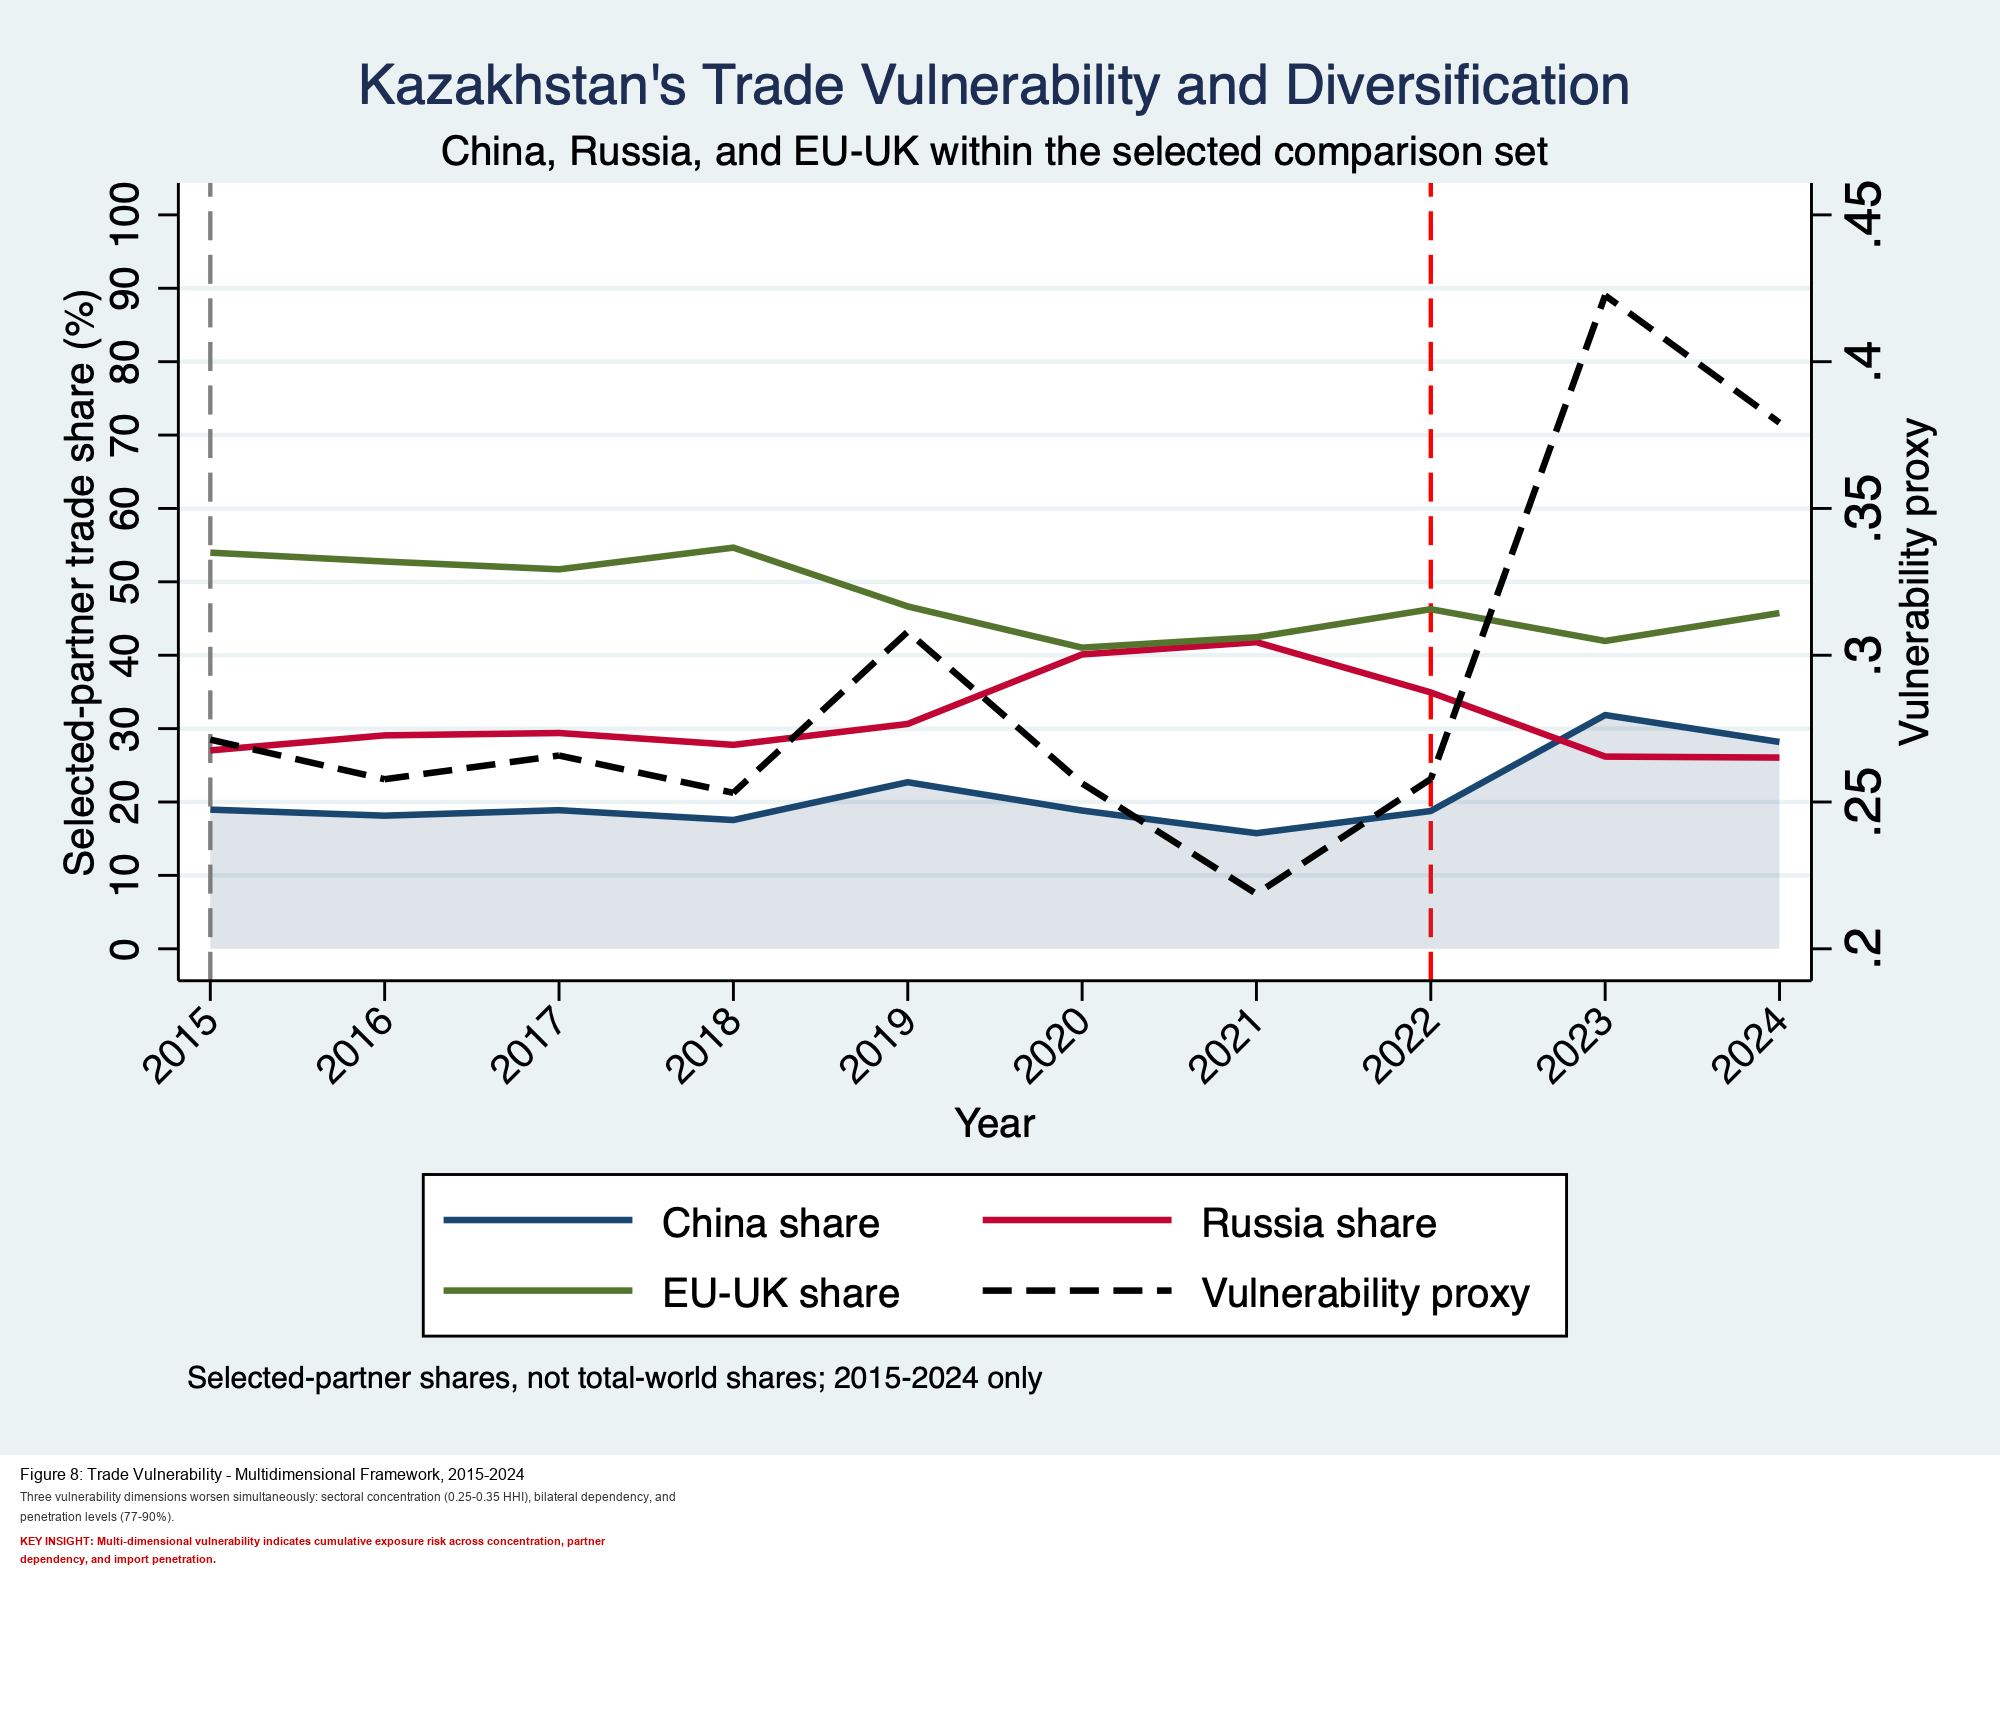
\includegraphics[width=0.92\textwidth]{figures/fig8_vulnerability_multivector_annotated.png}
\caption{Multivector trade-share dynamics: EU, Russia, China comparison, 2015--2024. Source: own calculation from WITS data.}
\label{fig:ii2a}
\end{figure}

\begin{figure}[H]
\centering
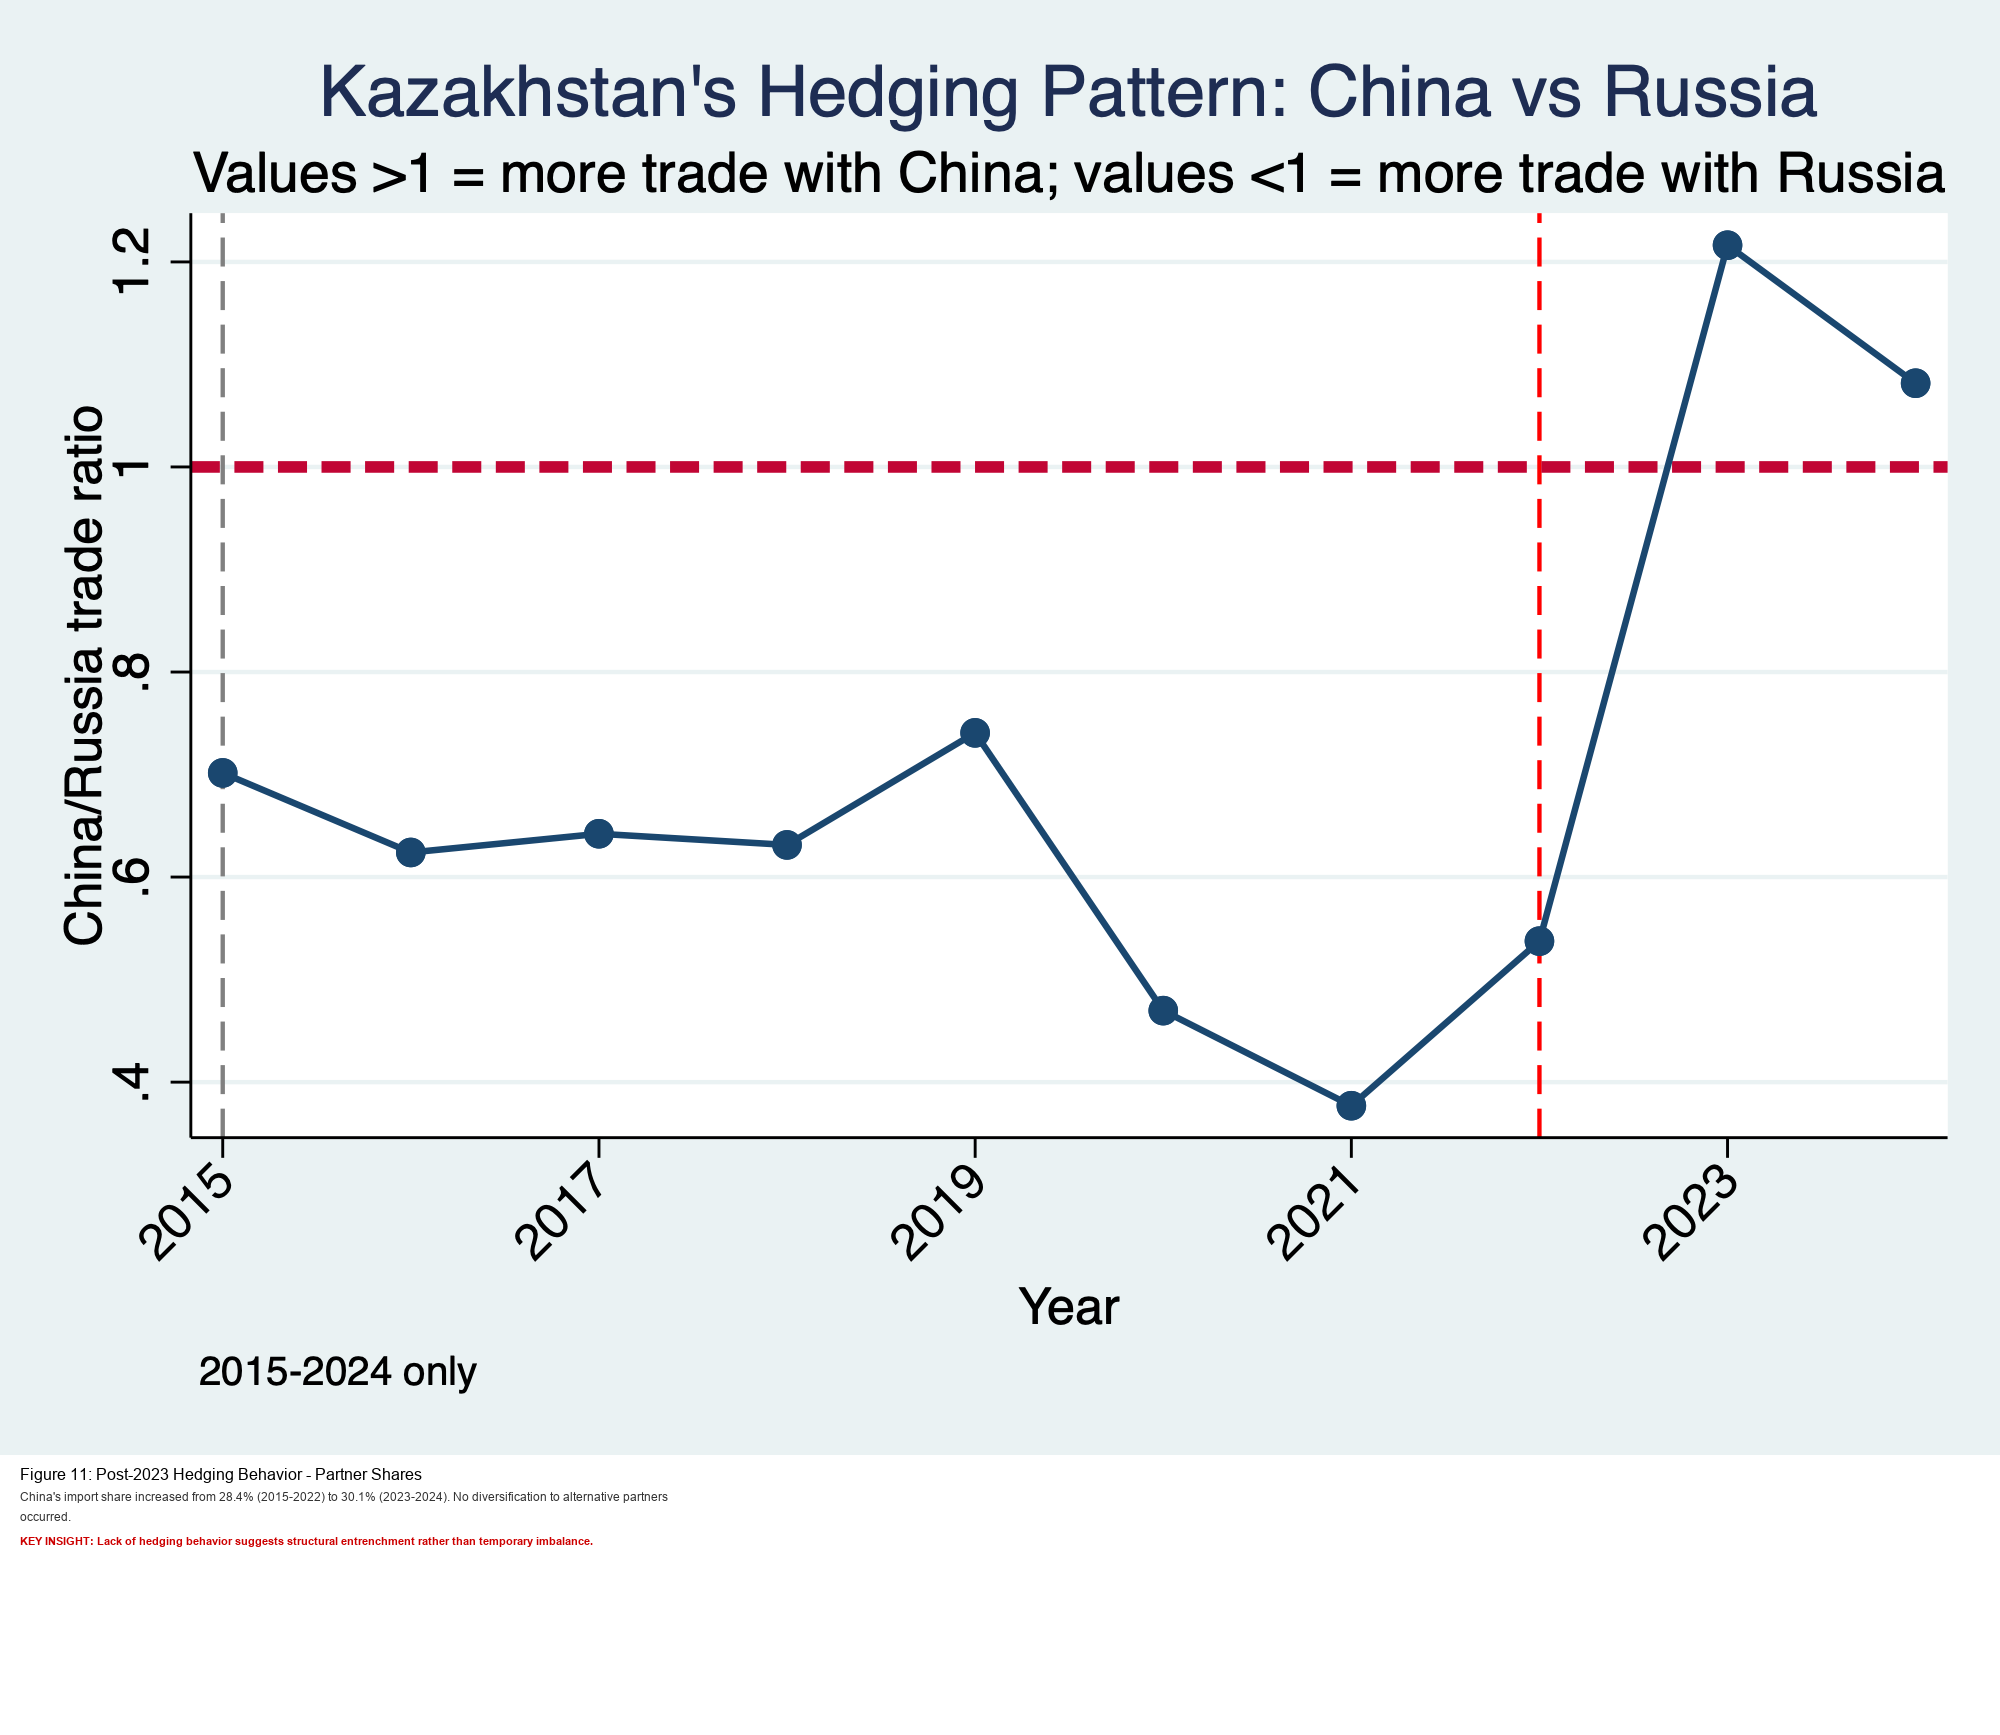
\includegraphics[width=0.92\textwidth]{figures/fig11_hedging_behavior_annotated.png}
\caption{China--Russia comparative trade orientation, 2015--2024. Source: own calculation from WITS data.}
\label{fig:ii2b}
\end{figure}

\begin{table}[H]
\centering
\small
\caption{Kazakhstan--China Annual Bilateral Trade, 2015--2024 (US\$ billions)}
\label{tab:annual_trade}
\begin{tabular}{lrrrr}
\toprule
Year & Exports & Imports & Balance & Total \\
\midrule
2015 & 10.96 & 10.18 & +0.78 & 21.14 \\
2016 & 8.43  & 7.33  & +1.10 & 15.75 \\
2017 & 11.60 & 9.39  & +2.21 & 20.99 \\
2018 & 12.61 & 10.77 & +1.85 & 23.38 \\
2019 & 16.01 & 13.58 & +2.43 & 29.58 \\
2020 & 13.67 & 3.91  & +9.76 & 17.58 \\
2021 & 13.70 & 4.85  & +8.86 & 18.55 \\
2022 & 20.92 & 7.15  & +13.77& 28.07 \\
2023 & 29.52 & 33.54 & --4.03 & 63.06 \\
2024 & 29.79 & 30.31 & --0.51 & 60.10 \\
\bottomrule
\end{tabular}
\end{table}

%% ============================================================
%% VI. STRUCTURAL FEATURES OF SINO-KAZAKH TRADE
%% ============================================================
\section{Structural Features of Sino-Kazakh Trade}

\subsection{Three Phases of Bilateral Trade Dynamics}

The bilateral trade trajectory from 2015 to 2024 divides into three phases corresponding to distinct structural and geopolitical conditions (Figure~\ref{fig:ii1}). In the first phase, 2015--2019, total bilateral trade ranged from US\$15.75 billion to US\$29.58 billion, with Kazakhstan maintaining a modest annual surplus driven by commodity exports. This period is consistent with Lim et al.'s (2025) assessment that Kazakhstan had retained meaningful trade autonomy. In the second phase, 2020--2021, a pandemic-driven contraction pushed Chinese imports into Kazakhstan down to US\$3.9 billion in 2020, while Kazakhstani raw material exports declined less severely, reflecting the relative inelasticity of Chinese industrial demand for commodity inputs relative to consumer goods. In the third phase, 2022--2024, both export and import flows surged following the Ukraine invasion, but Chinese imports grew at a steeper rate than Kazakhstani exports, crossing the export line and producing a bilateral deficit for the first time in the series. Three factors drove the post-2022 import surge: rerouting of trade flows away from the Northern Corridor, Chinese manufacturers filling the market space vacated by sanctioned Russian and European suppliers, and the rapid expansion of Chinese automotive brands in Kazakhstan's consumer market (Figure~\ref{fig:iii1}).

\begin{figure}[H]
\centering
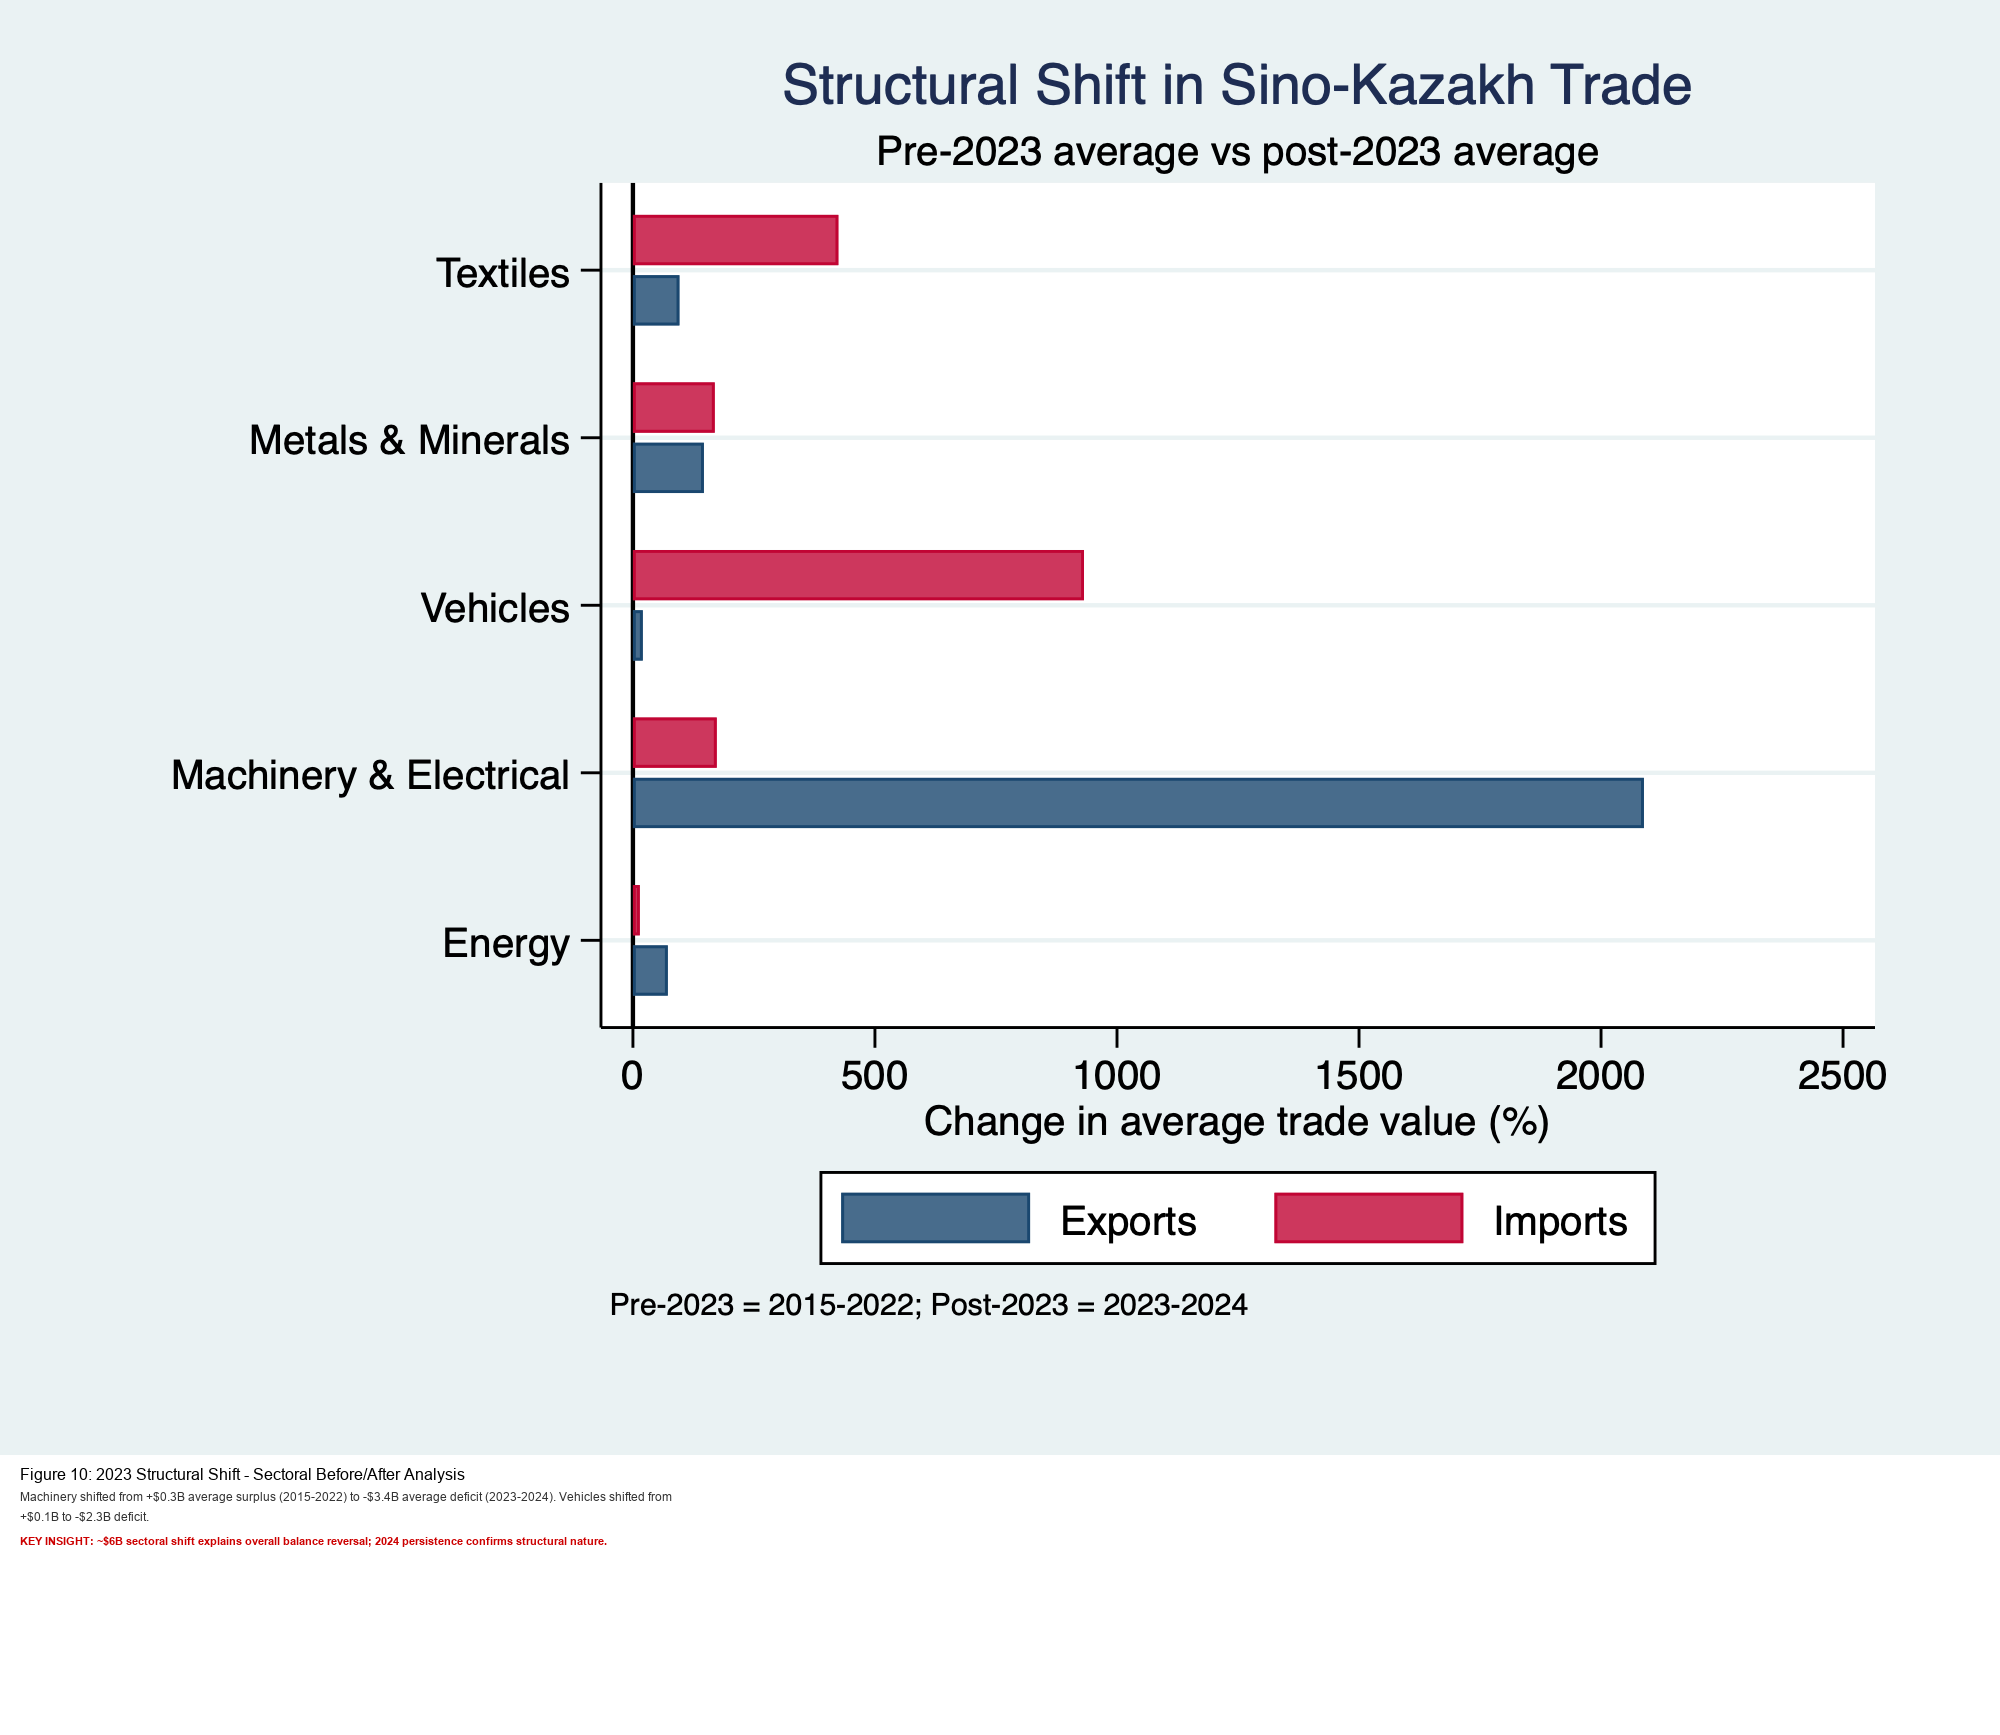
\includegraphics[width=0.92\textwidth]{figures/fig10_2023_structural_shift_annotated.png}
\caption{Structural shift timing: the 2023 trade balance reversal. Source: own calculation from WITS data.}
\label{fig:iii1}
\end{figure}

\subsection{Sectoral Composition: The Commodity-Manufacture Divide}

The product composition of bilateral trade shows a persistent divergence in economic complexity between Kazakhstan's exports and its imports. In 2024, copper ore and refined copper together accounted for over US\$5.5 billion in Kazakhstani exports to China, crude petroleum contributed US\$1.89 billion, and gold, radioactive chemicals, and ferrous metals comprised most of the remainder (Figure~\ref{fig:iii2a}). Kazakhstan's bilateral export revenues are accordingly determined by global commodity prices and Chinese industrial demand conditions, neither of which Kazakhstani policymakers can influence directly. China's exports to Kazakhstan present a different profile: passenger vehicles (US\$1.05 billion in 2024), computers (US\$684 million), and telephones (US\$937 million) dominate, with Chinese brands including JAC Motors, Haval, and Chery having displaced European and Japanese competitors as BRI logistics infrastructure reduced costs and the 2022 disruption eliminated competing supply chains (Figure~\ref{fig:iii2b}). Kazakhstan supplying raw material inputs while China supplies value-added manufactured goods is the commodity-manufacture divide that dependency and core-periphery frameworks identify as a structural marker of asymmetric exchange. The asymmetry in this case operates at the level of economic complexity rather than trade volume.

\begin{figure}[H]
\centering
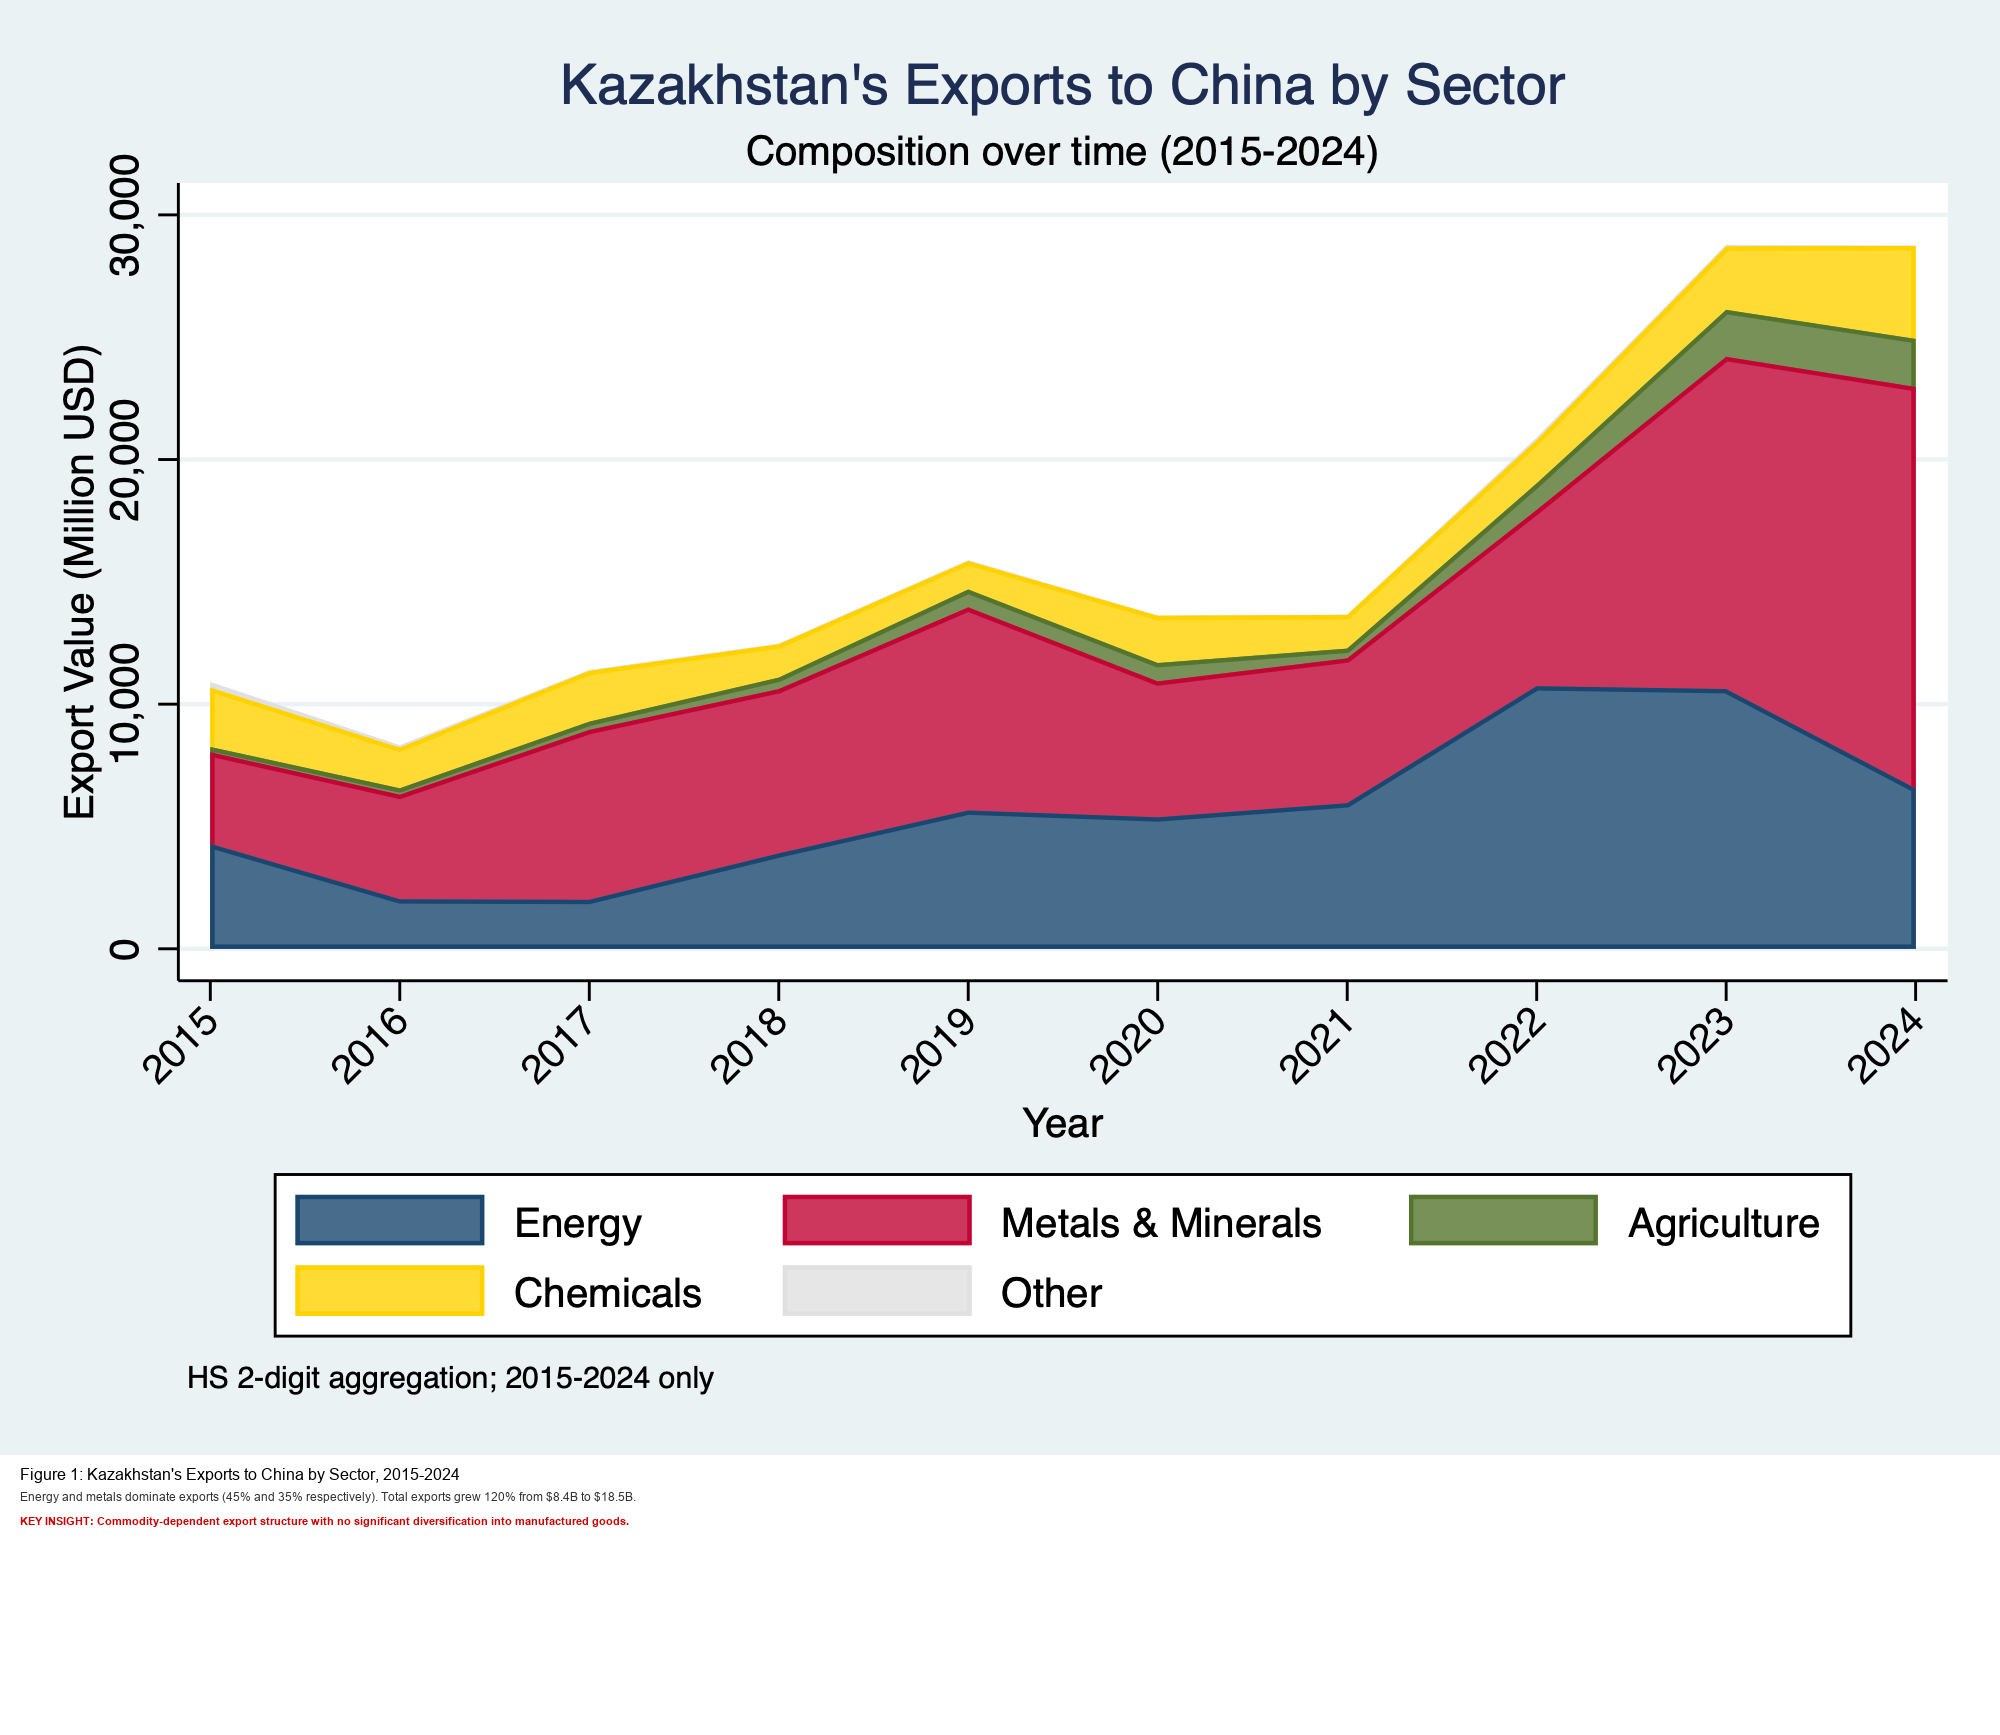
\includegraphics[width=0.92\textwidth]{figures/fig1_export_composition_annotated.png}
\caption{Kazakhstan's export composition to China by sector, 2012--2024. Source: own calculation from WITS HS-level data.}
\label{fig:iii2a}
\end{figure}

\begin{figure}[H]
\centering
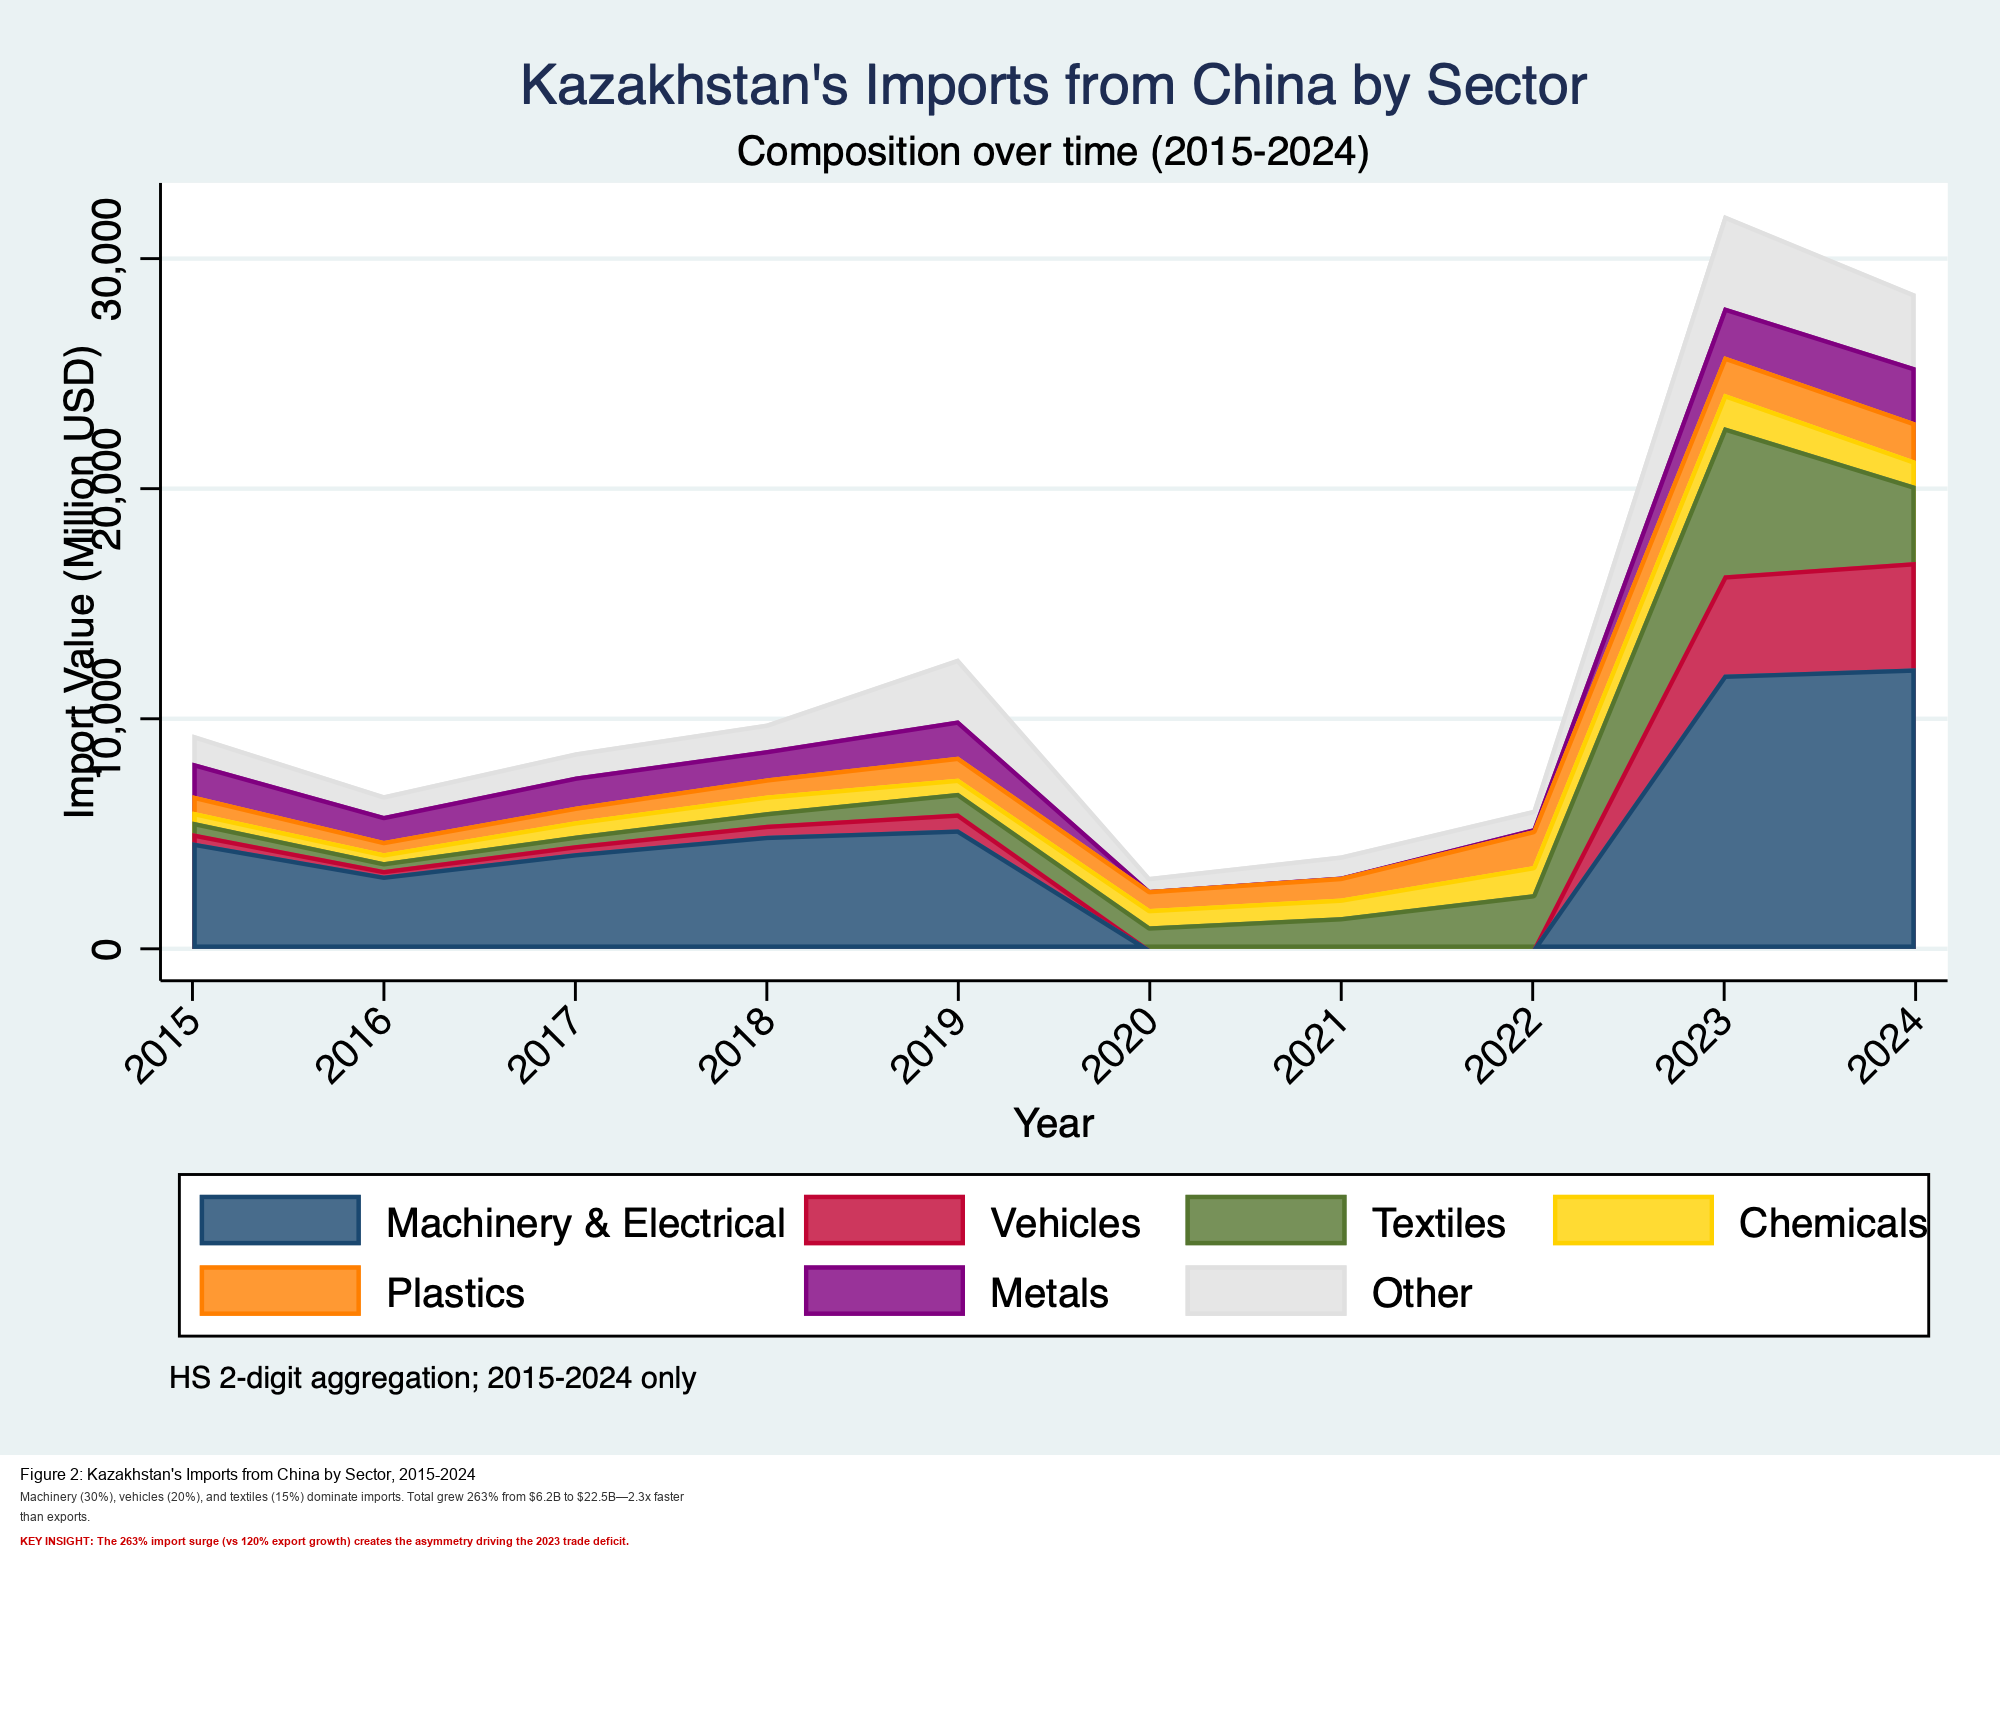
\includegraphics[width=0.92\textwidth]{figures/fig2_import_composition_annotated.png}
\caption{Kazakhstan's import composition from China by sector, 2012--2024. Source: own calculation from WITS HS-level data.}
\label{fig:iii2b}
\end{figure}

The RCA results confirm this structural reading. Kazakhstan's RCA scores above 1 in 2024 are confined to energy products (HS 27), base metals (HS 72--81), and ores (HS 26). Non-commodity sectors including machinery (HS 84--85), chemicals (HS 28--38), and transport equipment (HS 87) all show RCA scores below 1, with minimal change since 2015. Export growth across the period has been intensive -- greater volume in existing commodity categories -- rather than extensive, meaning entry into new product categories.

\subsection{The Accelerating Deficit}

For most of the BRI era, Kazakhstan maintained a modest bilateral surplus with China (Table~\ref{tab:annual_trade}), which provided diplomatic cover for the win-win framing promoted by both governments and supported the Lim et al. (2025) assessment that dependency had been avoided. The basis of this surplus was commodity price levels rather than productive competitiveness. The large surpluses of 2020--2022 reflect pandemic-era suppression of Chinese consumer goods exports rather than any improvement in Kazakhstan's economic position. The reversal came in 2023, when Chinese imports into Kazakhstan surged and the bilateral balance shifted to a deficit of US\$4.03 billion while Kazakhstani export revenue growth stalled. The deficit narrowed to US\$0.51 billion in 2024. The TAI series (Figure~\ref{fig:iii3b}) records a sharp positive shift in 2023--2024 that is discontinuous with the near-zero values of 2013--2019 and cannot be attributed to a cyclical movement, which points to a structural change in the bilateral trade dynamic.

\begin{figure}[H]
\centering
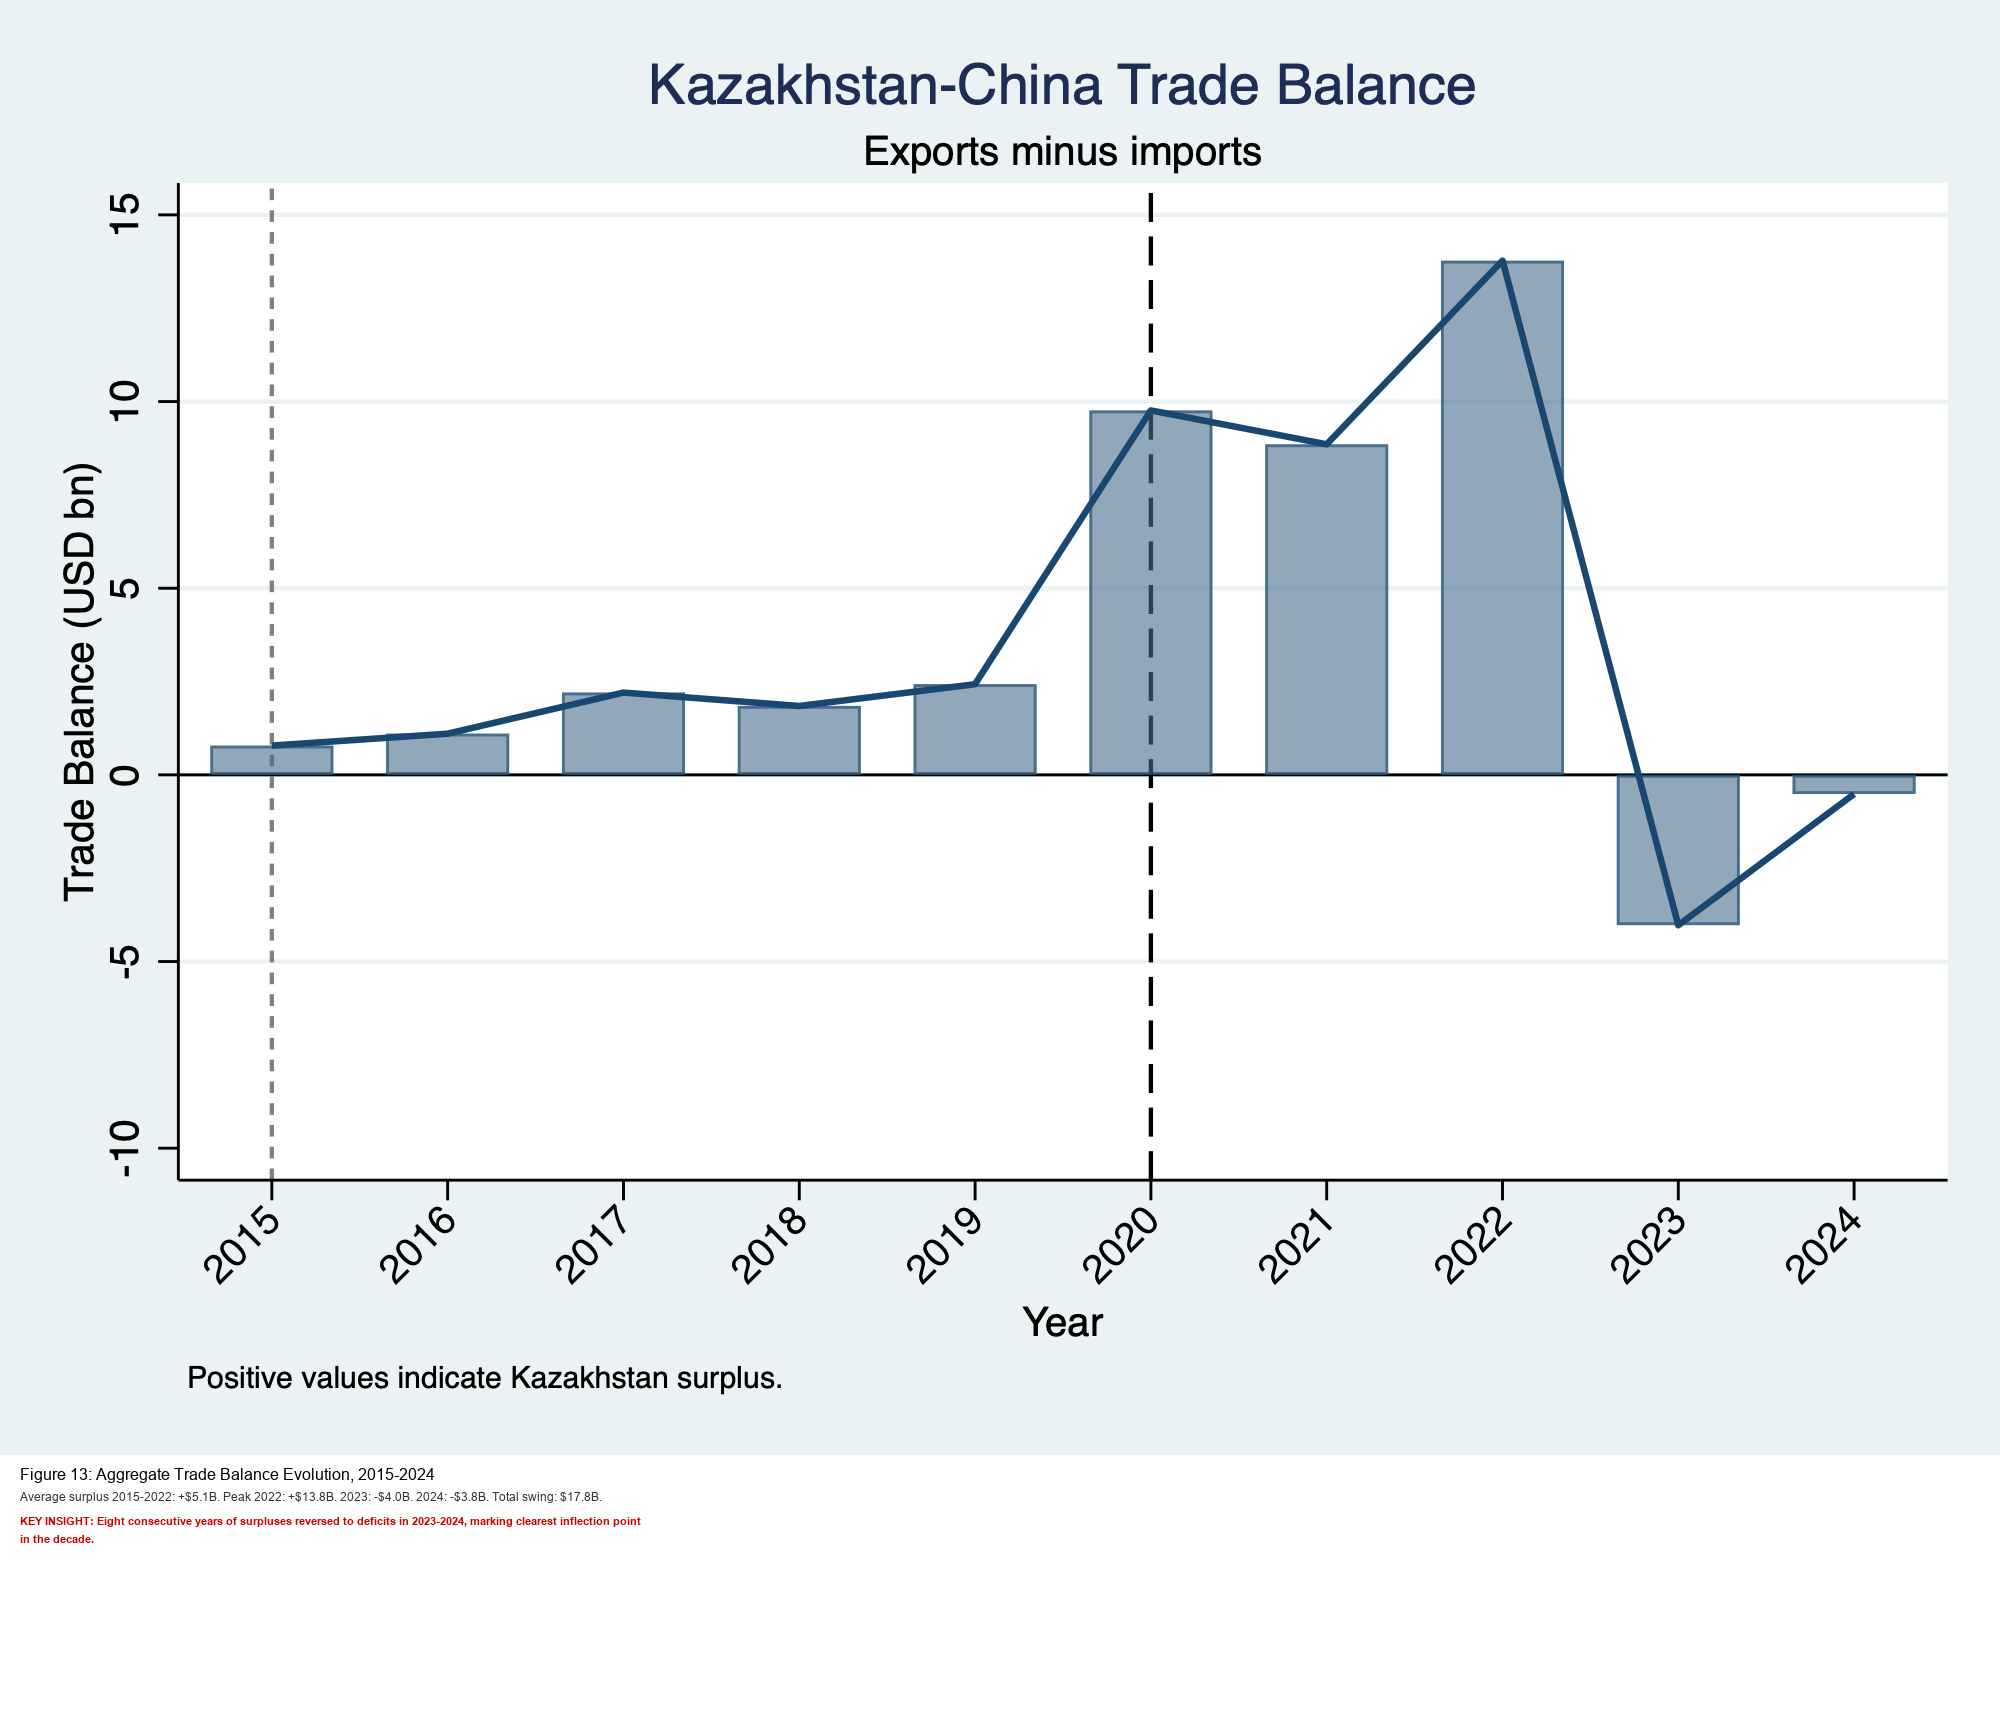
\includegraphics[width=0.92\textwidth]{figures/fig13_trade_balance_annotated.png}
\caption{Kazakhstan--China bilateral trade balance dynamics, 2015--2024. Source: own calculation from WITS data.}
\label{fig:iii3a}
\end{figure}

\begin{figure}[H]
\centering
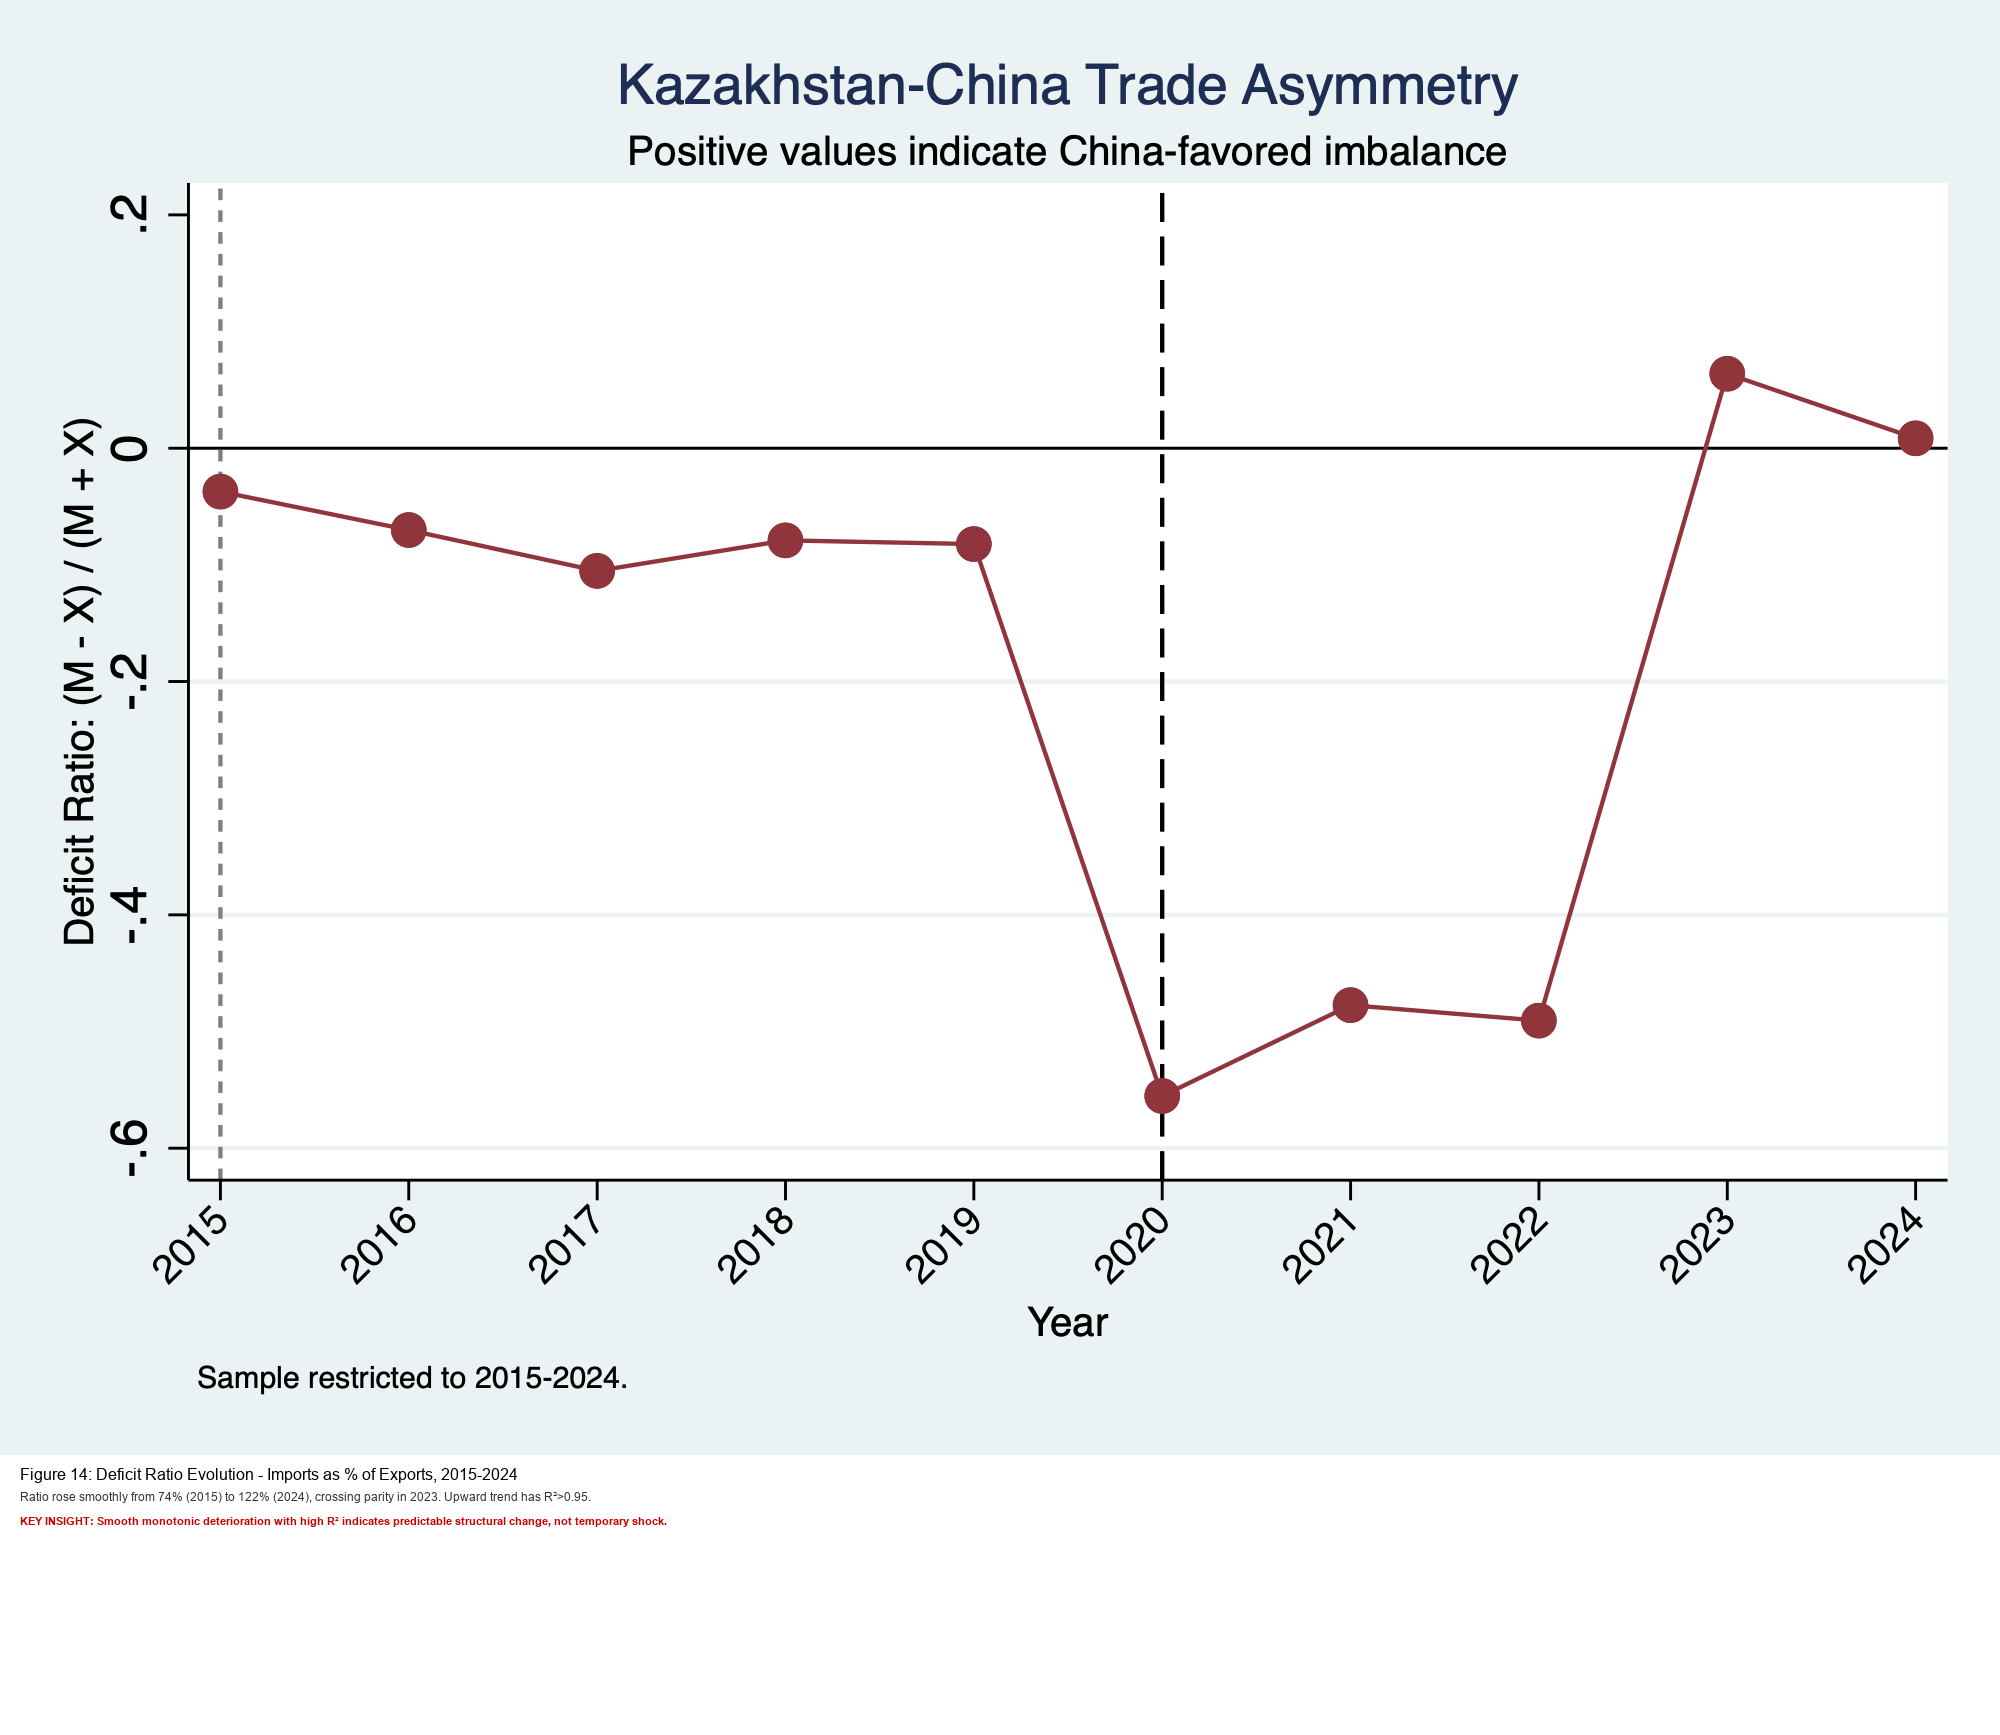
\includegraphics[width=0.92\textwidth]{figures/fig14_deficit_ratio_annotated.png}
\caption{Trade Asymmetry Index (TAI), Kazakhstan--China, 2013--2024. Positive values indicate import growth exceeding export growth. Source: own calculation from WITS data.}
\label{fig:iii3b}
\end{figure}

%% ============================================================
%% VII. COMPARATIVE ANALYSIS: CHINA, RUSSIA, AND THE EU
%% ============================================================
\section{Comparative Analysis: China, Russia, and the European Union}

\subsection{China versus Russia}

Kazakhstan's trade relationship with Russia is governed by the institutional architecture of the Eurasian Economic Union (EAEU), which establishes a common external tariff, harmonised regulatory standards, and a customs union framework. This regulatory integration is a mutual constraint: Kazakhstan cannot revise tariff schedules on Russian goods unilaterally without implicating its EAEU commitments. The product composition of Russian trade with Kazakhstan is relatively diversified, encompassing agricultural goods, construction materials, processed foods, and light manufactures in addition to energy, reflecting decades of Soviet-era industrial integration. China's trade relationship with Kazakhstan operates under a different institutional logic. Bilateral customs facilitation agreements and BRI investment frameworks improve transaction efficiency without producing the deep regulatory harmonisation of EAEU membership. This preserves greater formal policy flexibility for Kazakhstan while simultaneously generating structural dependencies through investment concentration and market penetration. China's position after 2022 as the primary beneficiary of Northern Corridor disruption means it absorbed market share previously held by Russian exporters without taking on the corresponding political and regulatory obligations of EAEU partnership (Figure~\ref{fig:ii2b}).

\subsection{China versus the European Union}

Kazakhstan's EU trade relationship is the most technologically asymmetrical of its three primary partnerships and the one most likely to generate productive upgrading incentives for Kazakhstani exporters. EU imports into Kazakhstan consist of precision machinery, capital goods, pharmaceutical products, and industrial equipment of significantly higher technological complexity than Chinese equivalents. The EU's regulatory framework, including the Carbon Border Adjustment Mechanism, creates compliance requirements for Kazakhstani exporters that the China--Kazakhstan trade architecture does not, and meeting those requirements builds regulatory and institutional capacity with spillover effects. The investment comparison further distinguishes the two partnerships. Chinese FDI in Kazakhstan reached US\$11.4 billion by end-2024, representing 32 per cent of China's total Central Asian investment. The sectoral composition shifted over the study period: extractive industries fell from 68 per cent to 54 per cent of Chinese FDI stock, manufacturing rose from 13 per cent to 22 per cent, and renewable energy from 4 per cent to 12 per cent. European FDI has been concentrated in finance, services, and technology transfer under stronger transparency and governance conditions. Kazakhstan has pursued a dual-track approach, accepting Chinese capital volumes while seeking alignment with EU standards in key export sectors. To date, the outcomes of this approach have favoured Chinese commercial penetration over the kind of productive upgrading associated with European investment conditions (Figure~\ref{fig:iv2a}).

\begin{figure}[H]
\centering
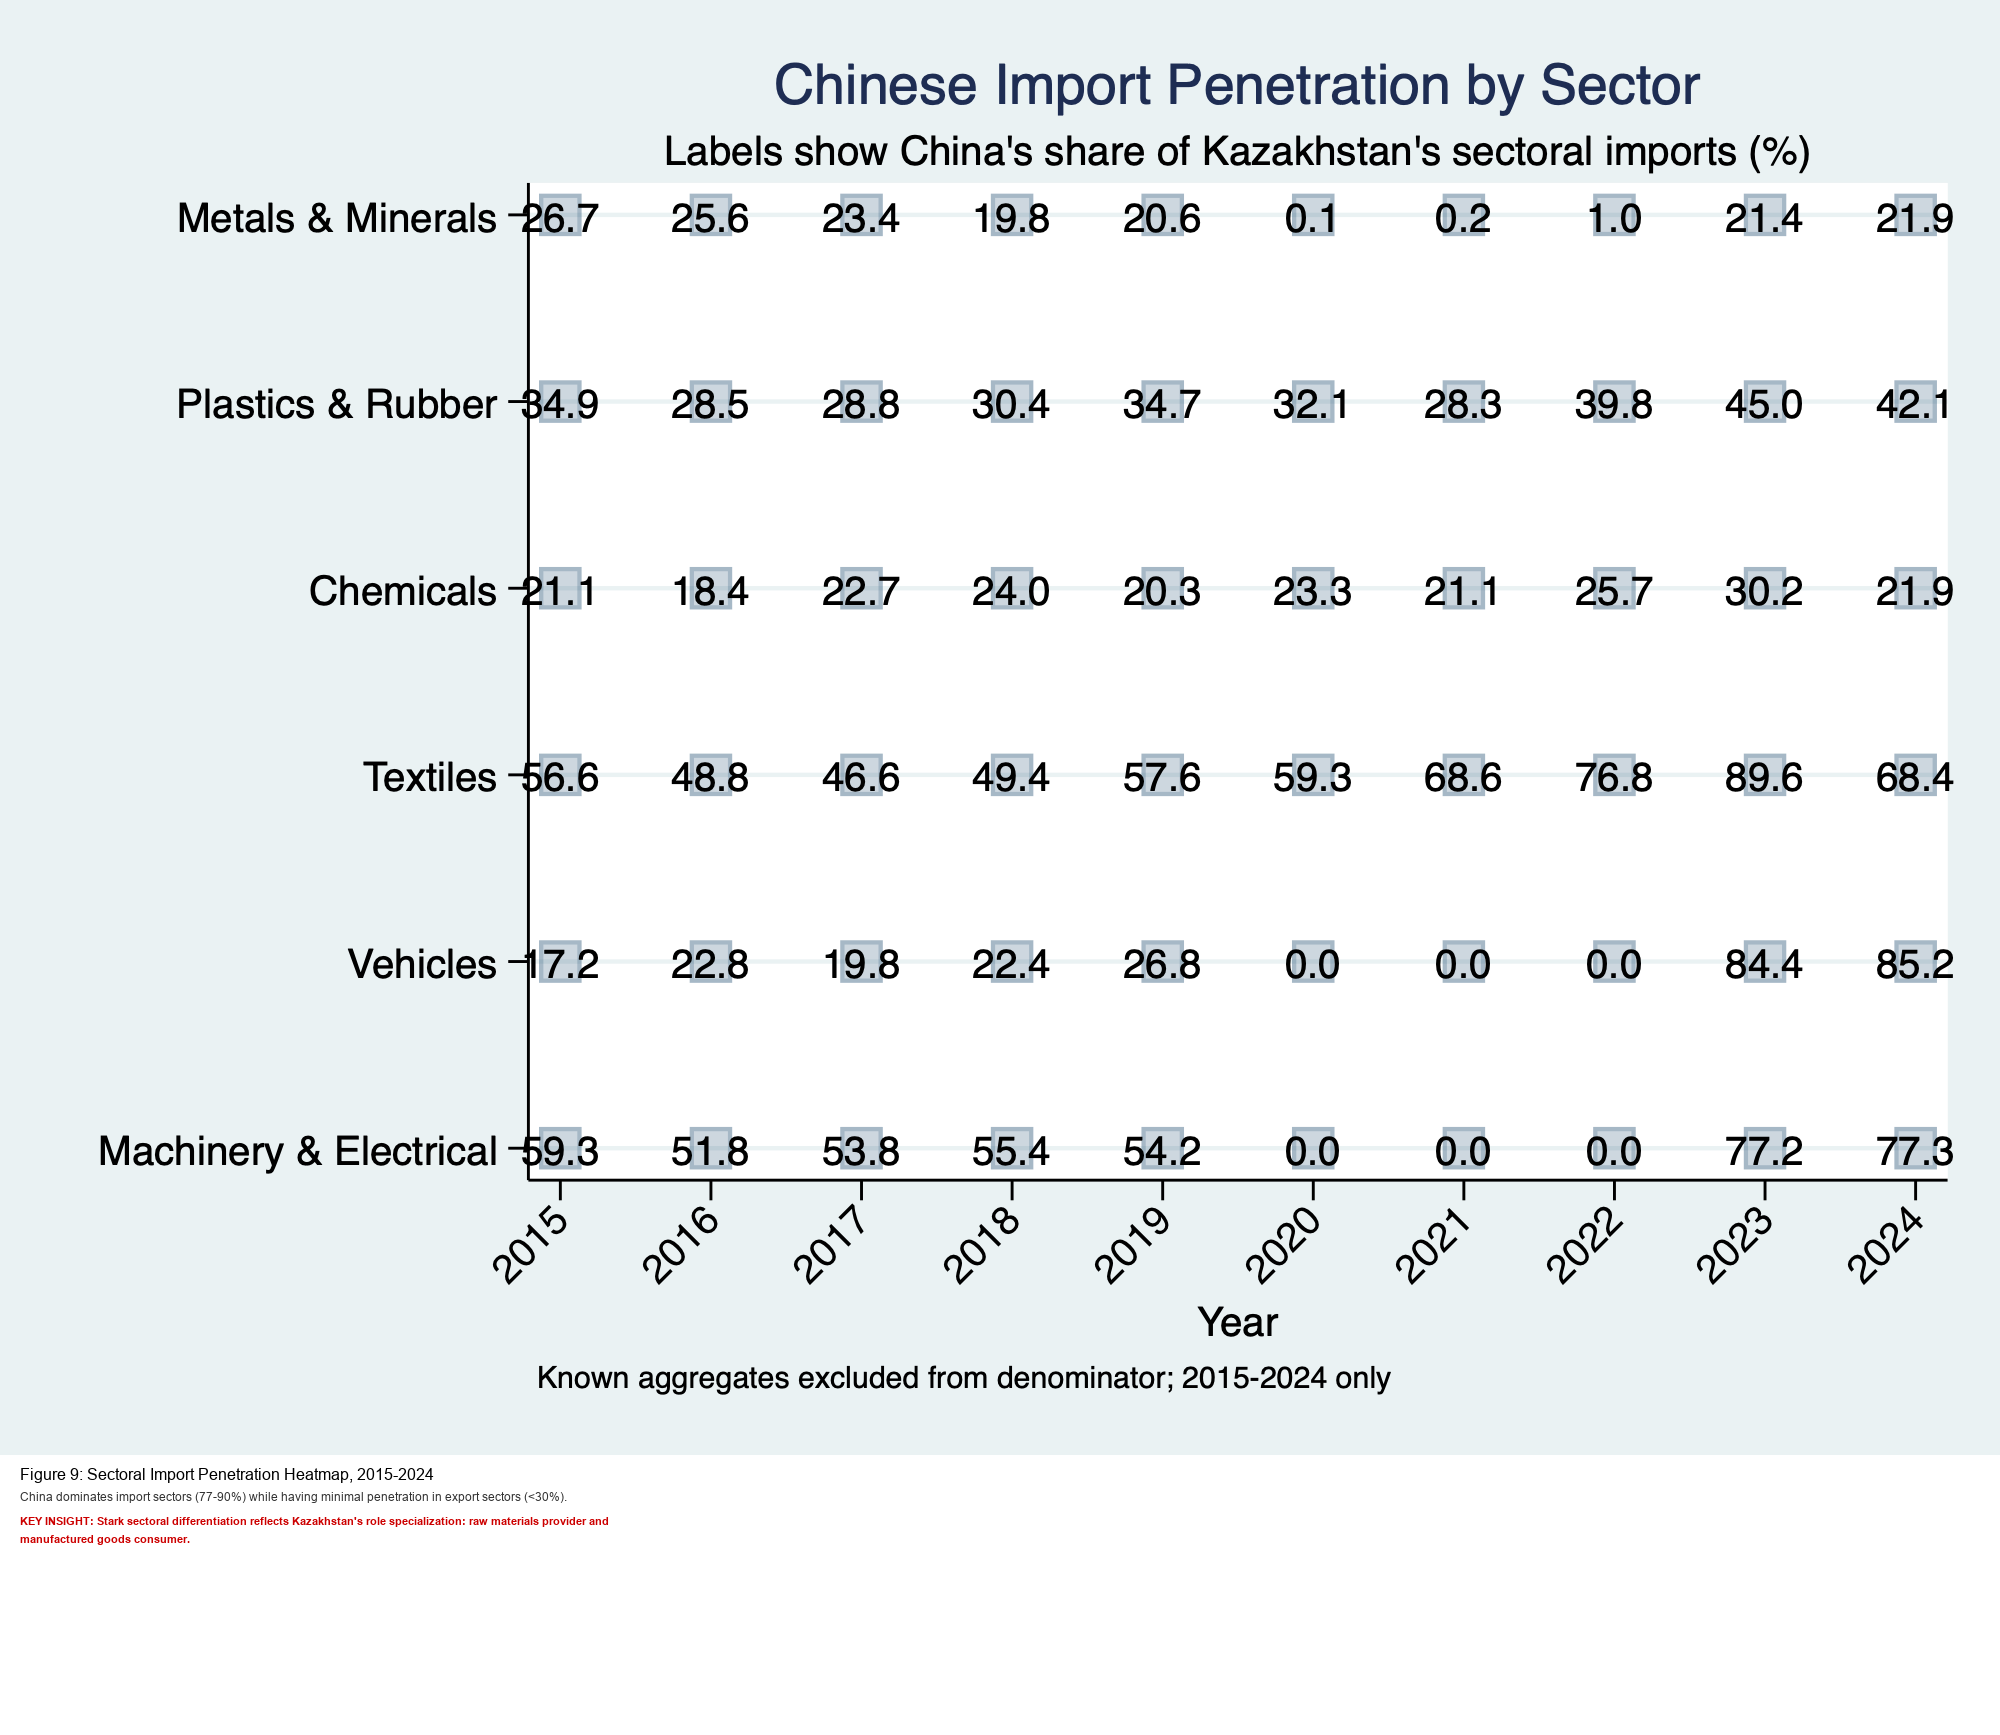
\includegraphics[width=0.92\textwidth]{figures/fig9_sectoral_penetration_heatmap_annotated.png}
\caption{Sectoral penetration comparison: China, Russia, EU in Kazakhstani import markets. Source: own calculation from WITS data.}
\label{fig:iv2a}
\end{figure}

\begin{figure}[H]
\centering
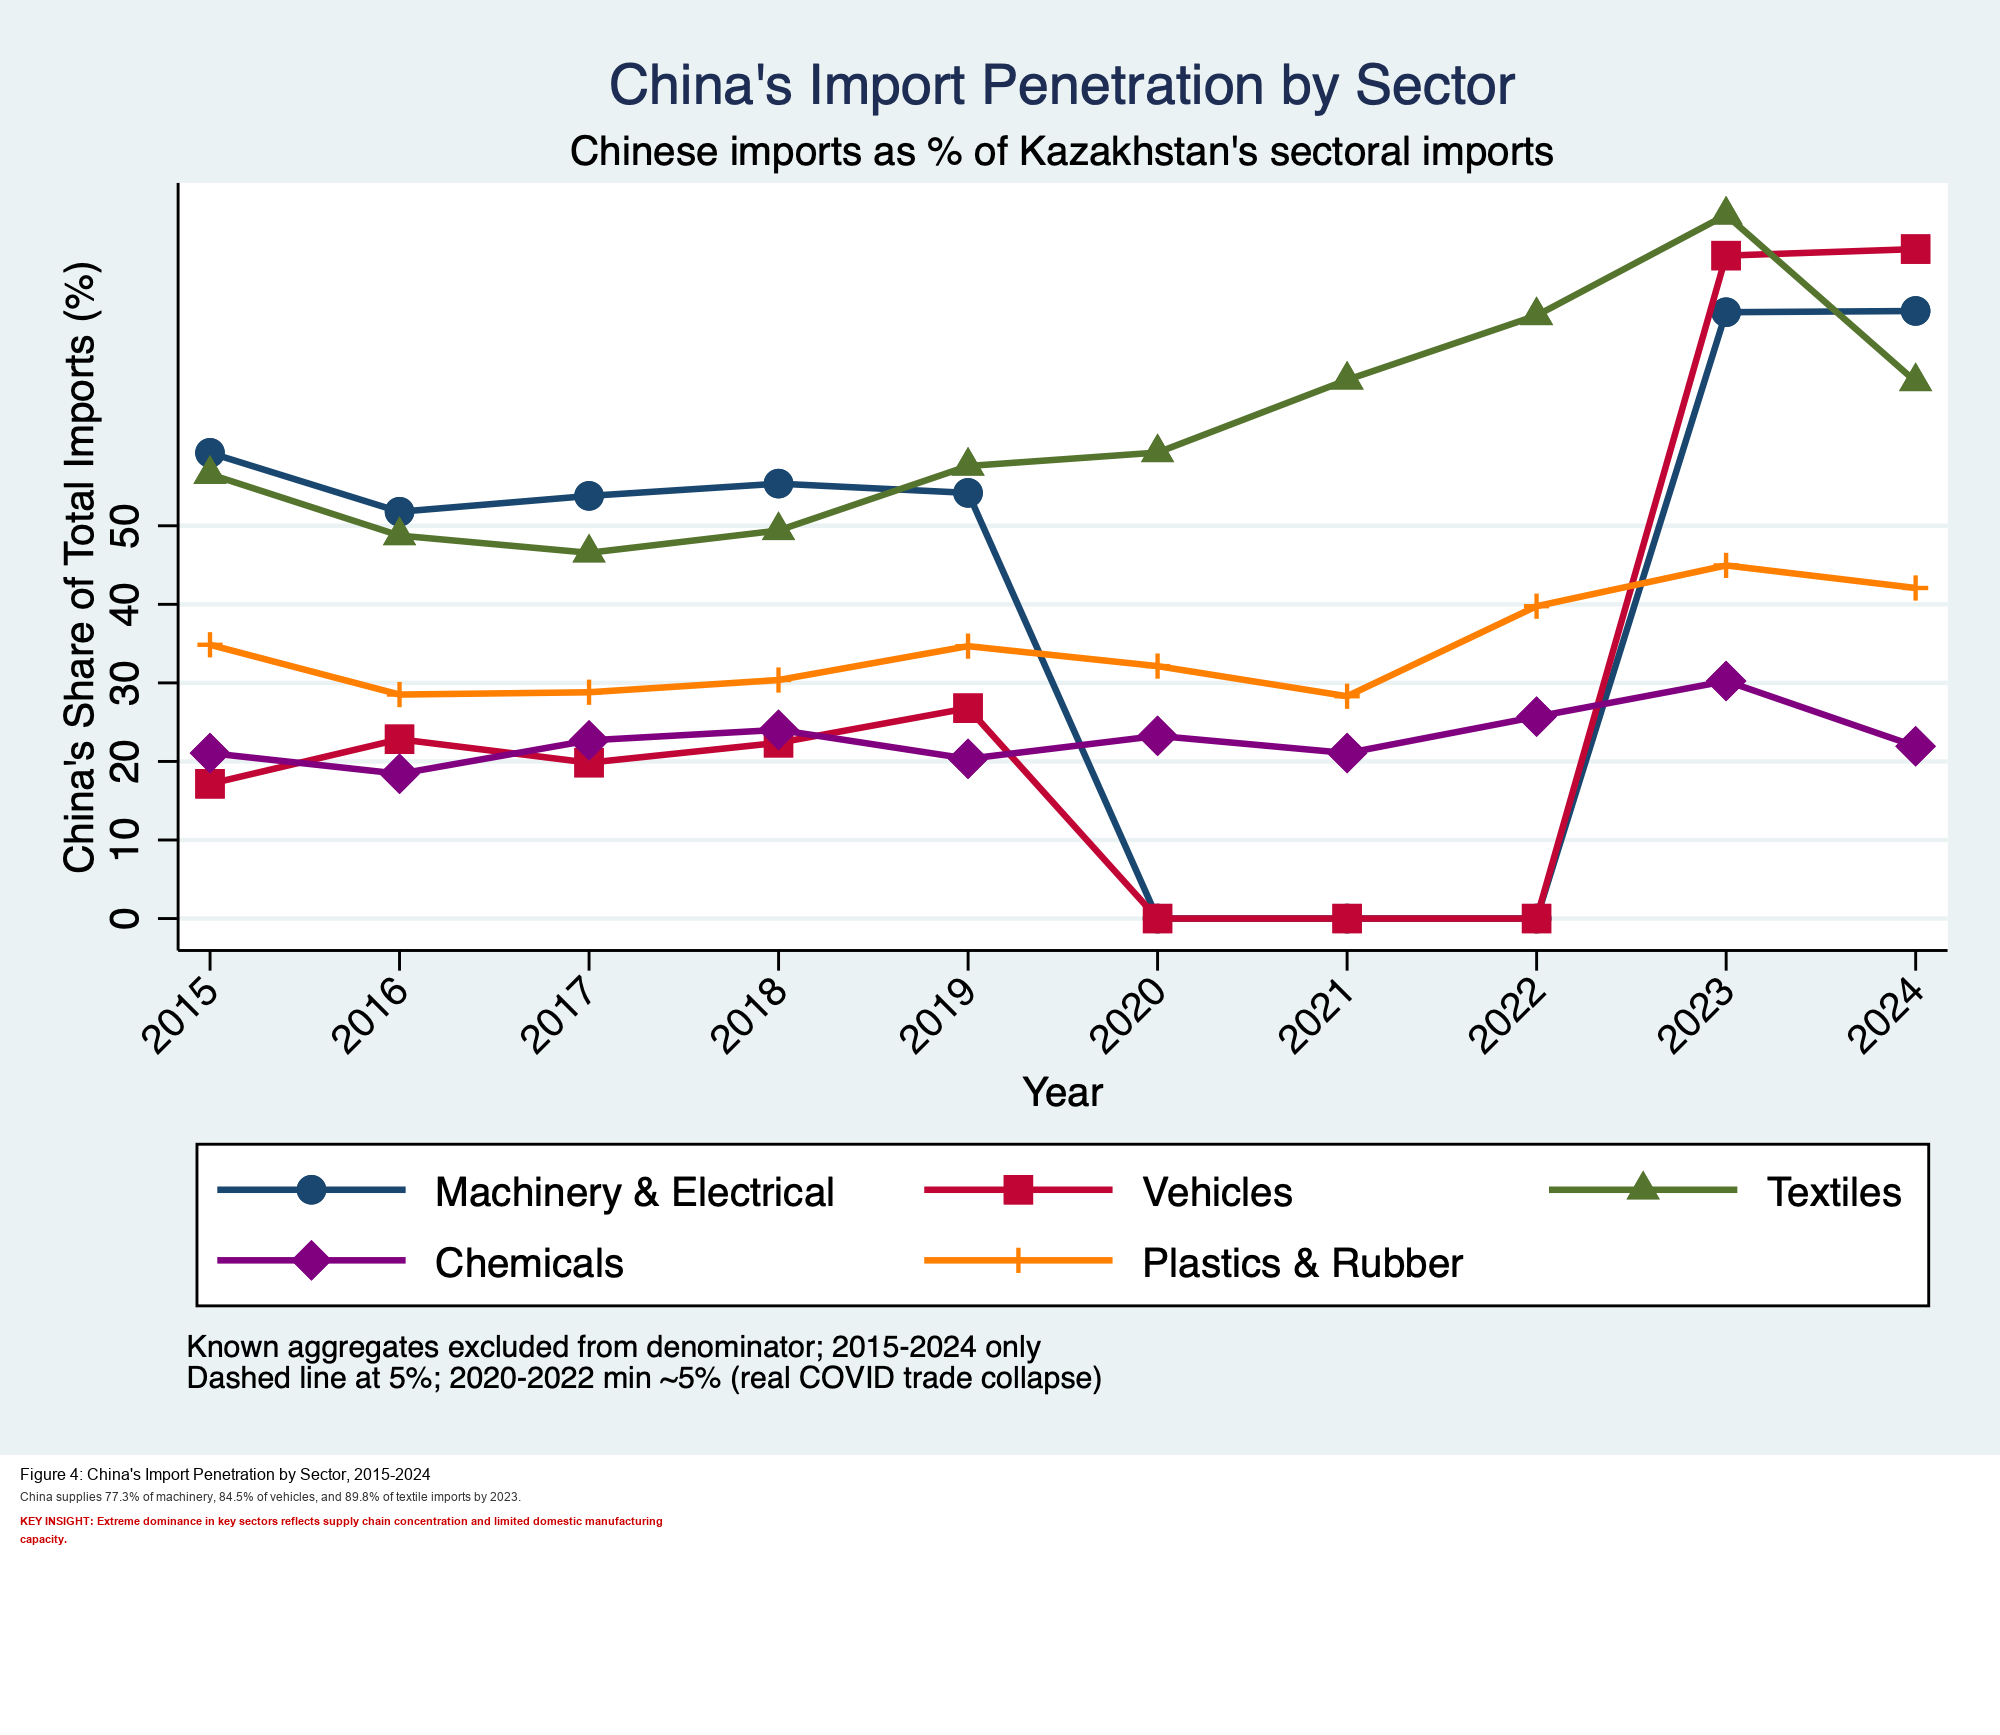
\includegraphics[width=0.92\textwidth]{figures/fig4_china_penetration_annotated.png}
\caption{China import penetration and perceived dependency risk, 2015--2024. Source: own calculation from WITS data.}
\label{fig:iv2b}
\end{figure}

\subsection{Deindustrialization Risk and Societal Constraints}

Among Kazakhstan's three major trading partners, the Sino-Kazakh relationship presents the most severe combination of dependency risks, because China's economic scale, competitive manufacturing position, and investment penetration operate across multiple sectors simultaneously rather than being confined to a single domain. The automotive sector is illustrative. Chinese manufacturers have used Kazakhstan's EAEU membership to establish assembly facilities that qualify for ``Made in Kazakhstan'' certification, gaining tariff-free access to Russian and Central Asian markets. The commercial benefit of this arrangement accrues primarily to Chinese original equipment manufacturers seeking EAEU market access, while Kazakhstan's position in the value chain is confined to lower-complexity assembly operations. Rather than developing an independent automotive supply chain, Kazakhstan has functioned as an institutional gateway for Chinese industrial expansion into the broader EAEU market.

These structural risks are compounded by domestic political constraints. Elite-level diplomatic accommodation of Chinese economic activity coexists with persistent and broad-based popular hostility toward it, which has repeatedly limited the government's room for manoeuvre. The 2016 land reform protests, sustained opposition to the ``55 Factories'' industrial investment plan, and public anger over the treatment of ethnic Kazakhs in Xinjiang have created a domestic environment in which the government must defend Chinese economic engagement while being unable to address the commodity-dependence and labour-market concerns that motivate public opposition. Neither administrative restrictions on Chinese investment nor government communications campaigns have resolved the underlying grievances. These constraints are likely to become more acute as the trade deficit deepens and Chinese commercial activity becomes more visible in domestic consumer markets (Primiano and Kudebayeva, 2025; MERICS, 2022).

%% ============================================================
%% VIII. SYNTHESIS AND CONCLUSIONS
%% ============================================================
\section{Synthesis and Conclusions}

The evidence assembled across the preceding sections points to a consistent conclusion. Between 2015 and 2024, Kazakhstan--China economic relations shifted from a condition of relative bilateral balance toward one of deepening structural asymmetry. The Trade Intensity Index crossed above parity for the first time in 2023 and remained elevated in 2024, indicating that bilateral trade is now more concentrated relative to Kazakhstan's global trade position than market-share fundamentals would predict. The RCA analysis shows no meaningful change in export structure over a decade of BRI investment. The Trade Asymmetry Index records a sharp and persistent positive shift from 2023 onward that is inconsistent with a cyclical explanation and is better explained by a structural break in the bilateral trade dynamic following the geopolitical disruption of Eurasian trade flows after 2022. The bilateral trade deficit, which did not exist before 2023, persisted through 2024 on an elevated import baseline.

These findings bear on the theoretical debate between complex interdependence and asymmetric dependence, and they suggest that the two frameworks address different aspects of the same relationship rather than competing explanations. Keohane and Nye's (1977) account correctly identifies the structural condition. The Sino-Kazakh relationship exhibits all three characteristics of complex interdependence: multiple channels -- energy pipelines, BRI investment, Trans-Caspian transit, and consumer goods supply chains -- connect the two economies simultaneously; the issue hierarchy in bilateral negotiations has shifted so that logistical access and trade facilitation take precedence over sovereignty protection; and Kazakhstan has no military instrument available to alter the commodity-manufacture terms of bilateral exchange. These conditions mean that the costs of exit are prohibitive and that Kazakhstan cannot disengage from any single channel without incurring costs across the others.

The sensitivity-vulnerability distinction, however, is where the 2023--2024 data provide the more precise theoretical finding. Through 2022, Kazakhstan was sensitive to Chinese demand conditions -- commodity price cycles and Chinese industrial output fluctuations transmitted rapidly into the bilateral trade balance -- but retained some capacity to adjust through its multivector diplomatic portfolio. The 2023 import surge established a new structural baseline that has not reversed. Kazakhstan has not visibly adjusted its export composition or reduced its import exposure in the period since. This is consistent with a transition from sensitivity to vulnerability in Keohane and Nye's terms: the costs of interdependence have become durable rather than transient, and the policy instruments available to Kazakhstan have not proved sufficient to reverse them.

Hirschman (1945) supplies the mechanism that explains why this transition occurred. Kazakhstan's alternative partners have not expanded in proportion to China's growing share of its trade and investment. The commodity-manufacture divide means the terms of bilateral exchange have been deteriorating from Kazakhstan's perspective regardless of the diplomatic activity conducted at the elite level. The bilateral instruments deployed over the decade -- co-investment declarations, localisation roadmaps, corridor expansion agreements -- deepened the channels of the relationship without generating the productive diversification that would have been necessary to convert sensitivity into manageable vulnerability. The two theoretical frameworks together yield a cleaner conclusion than either does alone: complex interdependence describes why Kazakhstan cannot exit the relationship on acceptable terms, and Hirschman explains why the relationship's terms have been moving against Kazakhstan over time.

Kazakhstan's multi-vector foreign policy doctrine remains formally intact in diplomatic terms, but the structural conditions that give it substantive content are weaker than at any point in the post-independence period. Russia's strategic decline after 2022 did not diversify Kazakhstan's economic relationships; it concentrated them further around China, as Chinese manufacturers absorbed market share from both Russian and Western suppliers simultaneously. Sustaining multivectorism as a substantive commitment rather than a diplomatic posture requires at minimum an industrial policy oriented toward entry into higher-complexity export categories where Kazakhstan can develop genuine comparative advantage, rather than simply expanding volume in existing commodity sectors.

The Kazakhstan case holds broader relevance for other small and medium commodity-dependent states managing economic integration with a dominant industrial partner. Aggregate trade figures tend to obscure structural asymmetry during periods of high commodity prices, when bilateral balances remain favourable. The asymmetry becomes visible when commodity price cycles turn and import penetration from the dominant partner accelerates simultaneously. Diplomatic mechanisms and institutional frameworks are a necessary component of any response, but they are not sufficient on their own. Without productive diversification that shifts the export structure toward higher-value goods, smaller states remain exposed to the terms-of-trade deterioration that Hirschman's thesis anticipates, irrespective of the sophistication of their hedging strategies.

%% ============================================================
%% REFERENCES
%% ============================================================
\section*{References}

\begin{flushleft}
Amineh, M. P., \& Li, S. (2025). The structural challenges of transnationalizing the China-led BRI: The case of Pakistan. \textit{Journal of Contemporary Asia}. \url{https://doi.org/10.1177/0169796X251369694}

Balassa, B. (1965). Trade liberalisation and ``revealed'' comparative advantage. \textit{The Manchester School}, 33(2), 99--123.

Bitabarova, A. U. (2018). Unpacking Sino-Central Asian engagement: The case of Kazakhstan. \textit{Asian Security}, 14(1), 30--55.

Bitabarova, A. U. (2019). Kazakhstan's perspective on the Belt and Road Initiative. \textit{Asian Studies Review}, 43(4), 595--613.

Blackwill, R. D., \& Harris, J. M. (2016). \textit{War by other means: Geoeconomics and statecraft}. Harvard University Press.

Brown, A. J. (1949). \textit{Applied economics: Aspects of the world economy in war and peace}. George Allen \& Unwin.

Cannon, B. J., \& Rossiter, A. (2025). Rethinking and arresting Eurasian hegemony: The centrality of Central Asia to Indo-Pacific strategies. \textit{International Affairs}, 101(4), 1193--1212.

Caspian Policy Center. (2023). \textit{China-Kazakhstan bilateral relations}. \url{https://www.caspianpolicy.org}

Castellano, A., \& Castillo, R. (2024). Chinese state capital as a partner for resource-based structural transformation? The Belt and Road Initiative and downstream linkages in Bolivia and Kazakhstan. \textit{The European Journal of Development Research}. \url{https://doi.org/10.1057/s41287-024-00640-1}

Chen, X., et al. (2025). The influence of the Belt and Road Initiative on China's advancement in global value chains and developing economies: A systematic review. \textit{The Chinese Economy}, 58(4), 87--114.

Clarke, M. (2015). Kazakhstan's multi-vector foreign policy: Diminishing returns in an era of great power `pivots'? \textit{The Asan Forum}.

Contessi, N. P. (2015). Foreign and security policy diversification in Eurasia: Issue splitting, co-alignment, and relational power. \textit{Problems of Post-Communism}, 62(5), 299--311.

Georgia Foundation for Strategic and International Studies (GFSIS). (2025, March). \textit{Current trends in political and economic relations between China and Kazakhstan}. \url{https://gfsis.org}

Haji, A. A., \& Khattak, S. H. (2025). Geopolitical chessboard: China's Belt and Road Initiative and shifting power dynamics. \textit{Discover Global Society}. \url{https://doi.org/10.1007/s44282-025-00200-w}

Hirschman, A. O. (1945). \textit{National power and the structure of foreign trade}. University of California Press.

Kassenova, N. (2017). China's Silk Road and Kazakhstan's bright path: Linking dreams of prosperity. \textit{Asia Policy}, 24(1), 110--116.

Keohane, R. O., \& Nye, J. S. (1977). \textit{Power and interdependence: World politics in transition}. Little, Brown.

Laruelle, M., \& Peyrouse, S. (2012). \textit{The Chinese question in Central Asia: Domestic order, social change, and the Chinese factor}. Hurst \& Company.

Lim, G., Tjia, L. Y.-N., \& Murashkin, N. (2025). Opportunities and challenges of China's economic ties with Kazakhstan: Looking back to look forward. \textit{The Chinese Economy}, 58(1). \url{https://doi.org/10.1080/10971475.2024.2373643}

Luttwak, E. N. (1990). From geopolitics to geo-economics: Logic of conflict, grammar of commerce. \textit{The National Interest}, 20, 17--23.

Mercator Institute for China Studies (MERICS). (2022). \textit{Kazakhstan's three-way balancing act between competing powers is under pressure}. \url{https://merics.org}

Neafie, W. (2022). Producing the Eurasian land bridge: A case study of geoeconomic contestation in Kazakhstan. \textit{Geopolitics}, 29(1), 1--28.

Pepe, J. M. (2021). \textit{The Middle Corridor as part of China's Belt and Road Initiative}. MERICS.

Peyrouse, S. (2012). Central Asia's evolving foreign policy: Multi-vectorism, Russia, China, and the West. \textit{PONARS Eurasia Policy Memo No. 230}.

Primiano, C. B., \& Kudebayeva, A. (2025). A bumpy ride for China's Belt and Road Initiative in Kazakhstan: Findings from a university survey. \textit{Journal of Current Chinese Affairs}. \url{https://doi.org/10.1177/18681026231211354}

Rolland, N. (2017). \textit{China's Eurasian century? Political and strategic implications of the Belt and Road Initiative}. National Bureau of Asian Research.

Stronski, P., \& Sokolsky, R. (2024, May). China, Russia, and power transition in Central Asia. \textit{Foreign Policy Research Institute}. \url{https://www.fpri.org}

Summers, T. (2016). China's `New Silk Roads': Sub-national regions and networks of global political economy. \textit{Third World Quarterly}, 37(9), 1628--1643.

Vanderhill, R., Lutsevych, O., \& Buras, P. (2021). How Kazakhstan is navigating its relations with China. \textit{International Affairs}, 97(5), 1337--1354.

World Bank Group. (2020). \textit{The Belt and Road Initiative: Kazakhstan country case study}. World Bank.
\end{flushleft}

\end{document}
